Chương này trình bày quá trình cài đặt và triển khai hệ thống thực nghiệm, từ xây dựng hạ tầng, cấu hình môi trường, triển khai ứng dụng microservices đến mô phỏng lỗi và huấn luyện mô hình Reinforcement Learning. Các bước triển khai được mô tả nhằm làm cơ sở cho việc đánh giá hiệu quả của hệ thống ở chương tiếp theo.

\section{Tổng quan kiến trúc hệ thống thực nghiệm}

Trước khi đi vào từng lớp triển khai cụ thể, Hình \ref{fig:overall-system-architecture} trình bày kiến trúc tổng thể của môi trường thực nghiệm được sử dụng trong đồ án. Sơ đồ này mô tả xuyên suốt chuỗi thành phần từ lớp truy cập bên ngoài, lớp hạ tầng AWS, cụm Kubernetes chạy ứng dụng \textit{mini-ecommerce}, tác nhân RL, nền tảng gây lỗi Chaos Mesh, lớp quan sát hệ thống, cho tới các công cụ tự động hóa như Terraform, Ansible và K6.

\begin{figure}[htbp]
    \centering
    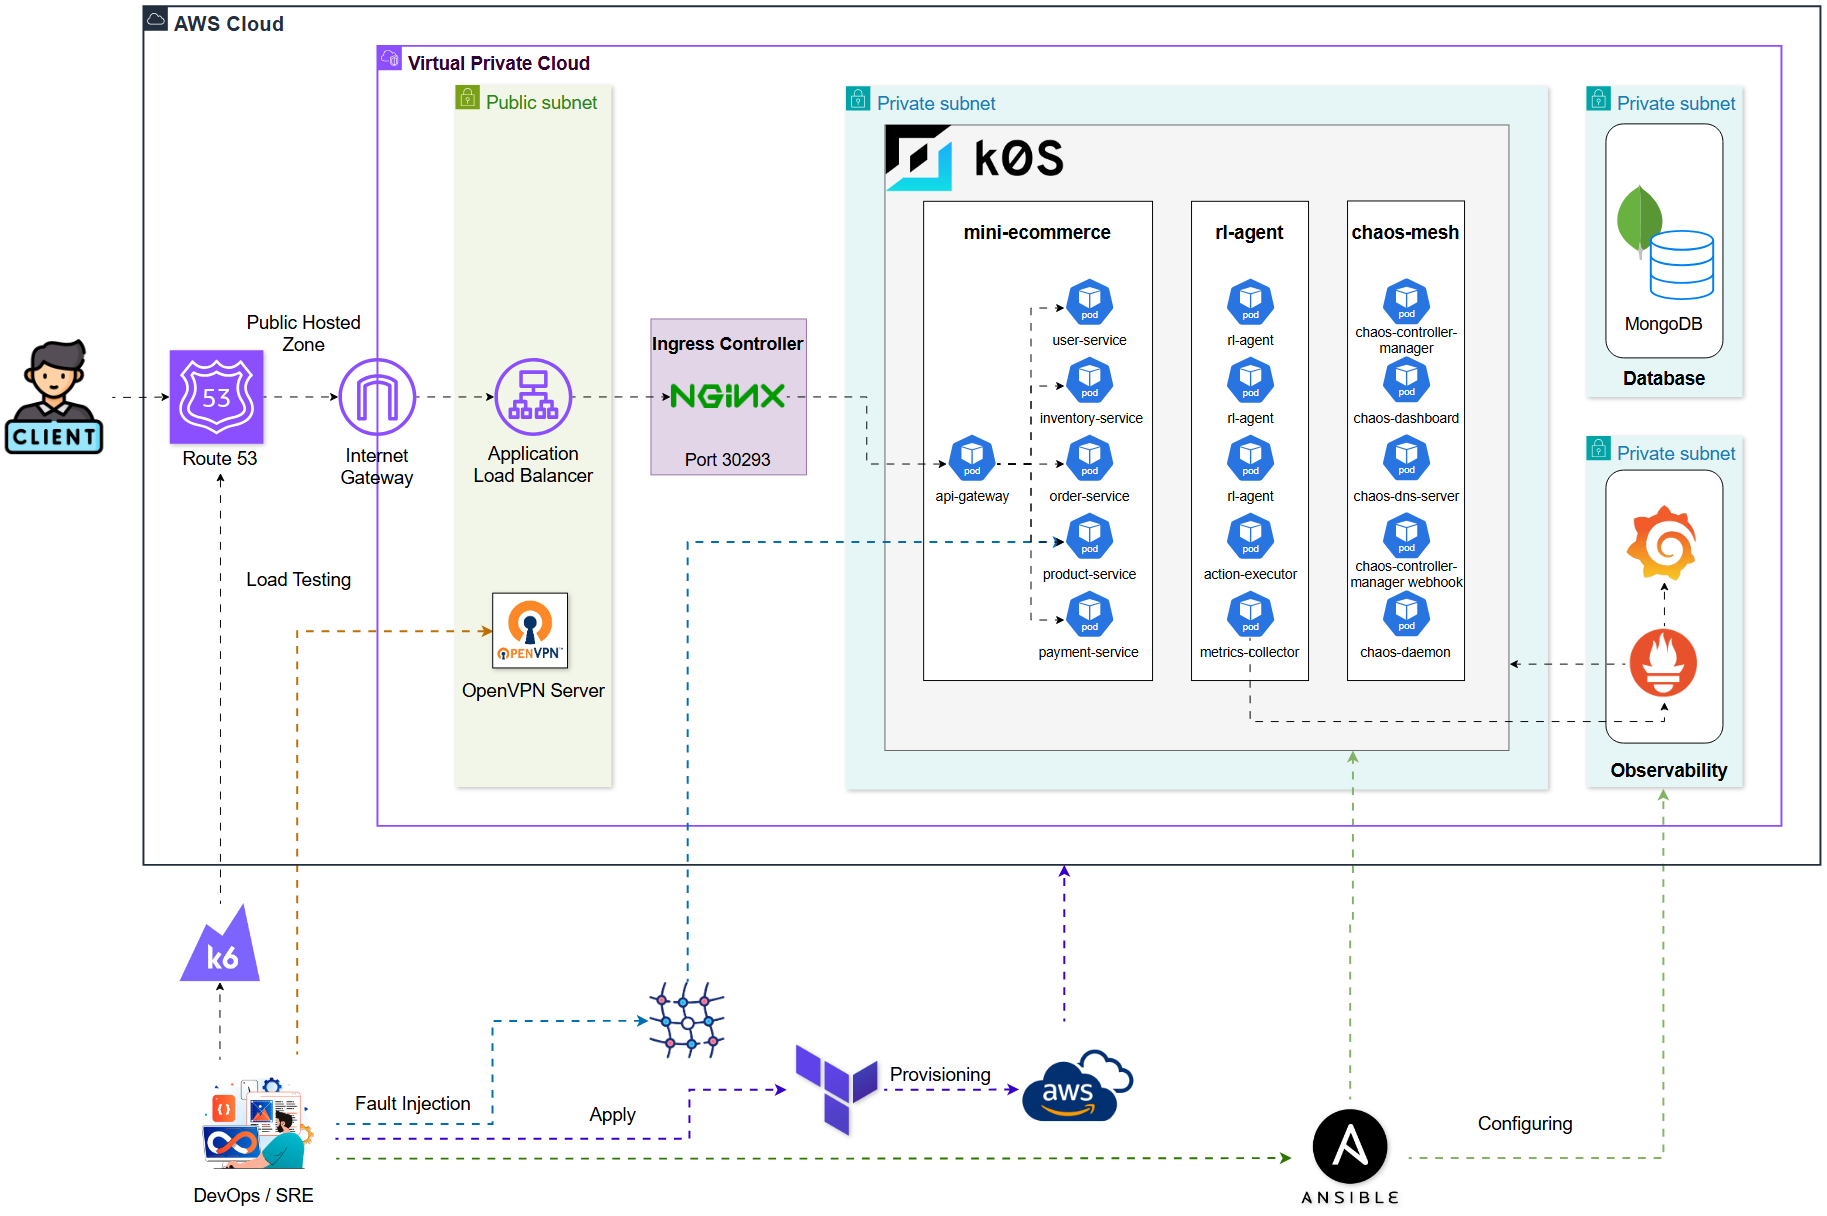
\includegraphics[width=1.0\textwidth]{graphics/chapter-5/5_0_architecture/architecture_diagram.png}
    \caption{Kiến trúc tổng thể môi trường triển khai và thực nghiệm của hệ thống}
    \label{fig:overall-system-architecture}
\end{figure}

\noindent Từ góc nhìn vận hành, người dùng và tải kiểm 
thử được định tuyến qua Route 53, Internet Gateway, 
Application Load Balancer và NGINX Ingress trước khi 
đi vào cụm \texttt{k0s}. Bên trong cụm, ứng dụng 
\textit{mini-ecommerce} đóng vai trò workload chính 
để sinh lưu lượng và sự cố phục vụ đánh giá khả năng 
tự phục hồi. Song song đó, namespace \texttt{rl-agent} 
đảm nhiệm việc thu thập trạng thái, suy luận hành động và 
thực thi can thiệp phục hồi, trong khi Chaos Mesh chịu 
trách nhiệm kích hoạt các kịch bản lỗi có kiểm soát.

\noindent Sơ đồ cũng cho thấy rõ mối liên hệ giữa các 
công cụ tự động hóa và giám sát trong toàn bộ pipeline 
triển khai. Terraform được sử dụng để khởi tạo tài nguyên 
trên AWS, Ansible tiếp tục cấu hình các máy chủ và dịch vụ 
nền, Prometheus/Grafana đảm nhiệm lớp observability, còn 
K6 cung cấp tải kiểm thử để tạo dữ liệu đánh giá. Nhờ đó, 
môi trường thực nghiệm không chỉ phản ánh cấu trúc triển 
khai thực tế mà còn hỗ trợ đầy đủ cho các pha benchmark, 
fault injection, thu thập metrics và đánh giá cơ chế 
self-healing dựa trên học tăng cường.

\section{Thiết kế cơ sở hạ tầng trên nền tảng AWS}

Môi trường thực nghiệm được thiết kế và triển khai trên 
nền tảng Amazon Web Services (AWS) nhằm đảm bảo tính linh 
hoạt, khả năng mở rộng tự động và mức độ sẵn sàng cao 
(High Availability). Kiến trúc hệ thống phân bổ dịch vụ 
trên nhiều Vùng khả dụng (Availability Zones - AZs) trong 
cùng một VPC (Virtual Private Cloud) để triệt tiêu các 
điểm lỗi đơn lẻ (SPoF) và tối ưu hóa khả năng chịu lỗi 
vật lý.

Chi tiết mô hình kiến trúc hạ tầng AWS được minh họa cụ thể trong Hình \ref{fig:aws-infra-architecture}.

\begin{figure}[htbp]
    \centering
    \includegraphics[width=1.0\textwidth]{graphics/chapter-5/cloud.png}
    \caption{Kiến trúc triển khai cơ sở hạ tầng trên nền tảng AWS}
    \label{fig:aws-infra-architecture}
\end{figure}

Kiến trúc hạ tầng bao gồm ba lớp chức năng chính:
\begin{itemize}
    \item \textbf{Lớp mạng (Networking Layer):} VPC dải 
    mạng \texttt{10.0.0.0/16} được chia làm các Public/Private 
    Subnet trên 03 AZs (us-east-1a, us-east-1b, us-east-1c). 
    Lớp này sử dụng Internet Gateway (IGW) cho kết nối ngoài, 
    NAT Gateway bảo mật cho phân vùng nội bộ, và Application 
    Load Balancer (ALB) điều phối lưu lượng từ phía người dùng 
    vào các dịch vụ bên trong hệ thống.
    \item \textbf{Lớp tính toán (Compute Layer):} Cụm Kubernetes được phân bổ trên cả 03 AZs để vận hành workloads. Trong đó, Master node đặt tại Private Subnet của AZ 1, các Worker node được phân tán ở các AZs khác nhau. Ngoài ra, hệ thống được bổ sung thêm Auto Scaling Group giúp hỗ trợ tăng giảm số máy Worker phục vụ lượng tải linh hoạt từ người dùng.
    \item \textbf{Lớp giám sát và quản trị (Management Layer):} Tích hợp Prometheus để thu thập dữ liệu huấn luyện (metrics) thời gian thực và Grafana để trực quan hóa phục vụ phân tích. Hệ thống quản trị được bảo mật thông qua OpenVPN Server đặt tại Public Subnet của AZ 3.
\end{itemize}

Để tối ưu hóa luồng lưu lượng và đảm bảo tính cô lập an toàn, 
địa chỉ IP được phân hoạch chi tiết cho toàn bộ các phân vùng 
mạng (Subnets) trong hệ thống như. Chi tiết được trình bày trong 
Bảng \ref{tab:subnet-ip-allocation}.

\begin{center}
\captionof{table}{Phân hoạch địa chỉ IP cho các Subnets trong hệ thống thực nghiệm}
\label{tab:subnet-ip-allocation}
\footnotesize
\renewcommand{\arraystretch}{1.0}
\begin{tabular}{|C{3.2cm}|C{2.8cm}|C{3.0cm}|L{6.0cm}|}
\hline
\textbf{Vùng khả dụng (AZ)} & \textbf{Loại Subnet} & \textbf{Dải địa chỉ (CIDR)} & \textbf{Thành phần được triển khai} \\ \hline
\multirow{3}{*}{us-east-1a (AZ 1)} & Public & 10.0.1.0/24 & ALB ENI, NAT Gateway \\ \cline{2-4} 
 & Private (k0s) & 10.0.11.0/24 & k0s Master, k0s Worker Node \\ \cline{2-4} 
 & Private (Data) & 10.0.21.0/24 & Prometheus, Grafana \\ \hline
\multirow{3}{*}{us-east-1b (AZ 2)} & Public & 10.0.2.0/24 & ALB ENI \\ \cline{2-4} 
 & Private (k0s) & 10.0.12.0/24 & k0s Worker Node (Auto Scaling) \\ \cline{2-4} 
 & Private (Data) & 10.0.22.0/24 & Phân vùng dự phòng (Unused) \\ \hline
\multirow{3}{*}{us-east-1c (AZ 3)} & Public & 10.0.3.0/24 & OpenVPN Access Server \\ \cline{2-4} 
 & Private (k0s) & 10.0.13.0/24 & k0s Worker Node \\ \cline{2-4} 
 & Private (Data) & 10.0.23.0/24 & Phân vùng dự phòng (Unused) \\ \hline
\end{tabular}
\end{center}

Cơ sở hạ tầng mạng và tính toán này thiết lập một môi 
trường thực nghiệm có tính chân thực cao, tương đương 
với các hệ thống Cloud Production. Đây là nền tảng cốt 
lõi để thực hiện các kịch bản kích hoạt sự cố nhân tạo 
(Chaos Injection) liên quan đến \textit{Pod failure}, 
từ đó đo lường chính xác thời gian phục hồi và độ ổn định 
của giải pháp đề xuất so với cơ chế mặc định của Kubernetes.

\section{Triển khai cơ sở hạ tầng sử dụng Terraform}

Để đảm bảo tính tự động hóa, tính nhất quán và khả năng tái lập nhanh chóng cho môi trường thực nghiệm, toàn bộ tài nguyên hạ tầng trên AWS được định nghĩa và khởi tạo dưới dạng mã nguồn (Infrastructure as Code - IaC) thông qua công cụ Terraform. Việc này giúp triệt tiêu các sai sót cấu hình thủ công và kiểm soát chặt chẽ trạng thái tài nguyên thông qua tệp tin \texttt{terraform.tfstate}.


Quy trình áp dụng hạ tầng được thực hiện qua các lệnh tiêu chuẩn của Terraform bao gồm: \texttt{terraform init} (khởi tạo môi trường), \texttt{terraform plan} (kiểm tra dự báo thay đổi) và \texttt{terraform apply} (thực thi khởi tạo thực tế trên AWS). 



\noindent Sau bước khởi tạo mã nguồn hạ tầng, tác giả tiến hành kiểm tra lại đầu ra của lệnh apply, trạng thái các máy ảo đang hoạt động và cuối cùng là cấu trúc mạng đã được dựng lên trên AWS để bảo đảm trạng thái triển khai khớp với thiết kế mong muốn.

\begin{center}
    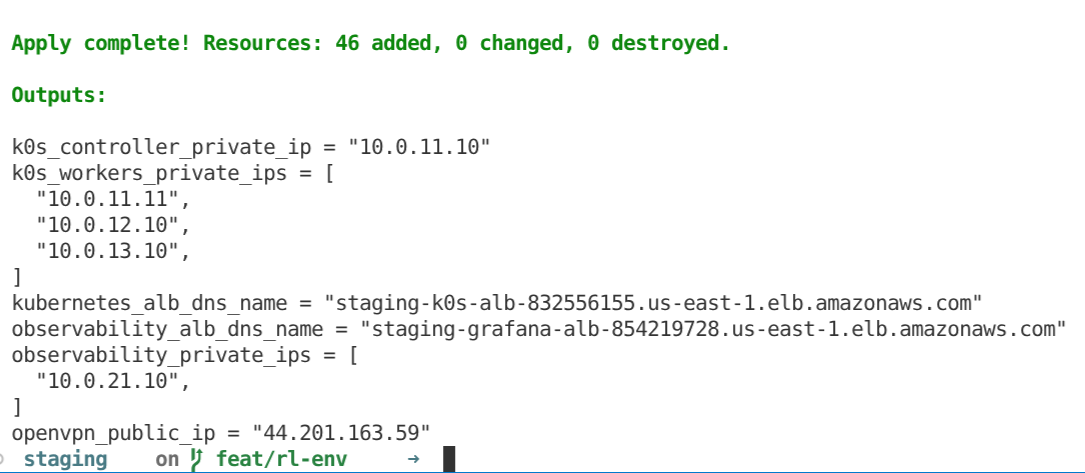
\includegraphics[width=0.92\textwidth]{graphics/chapter-5/5_1_infra/terraform_apply.png}
    \captionof{figure}{Đầu ra sau khi thực thi \texttt{terraform apply}}
    \label{fig:terraform-apply-output}
\end{center}

\noindent Hình \ref{fig:terraform-apply-output} ghi nhận kết quả \texttt{46 added, 0 changed, 0 destroyed}, cho thấy toàn bộ tài nguyên hạ tầng đã được tạo mới thành công và không phát sinh sai lệch trạng thái trong lần apply này. Các output quan trọng như địa chỉ IP private của controller, danh sách IP của các worker, DNS của Application Load Balancer và địa chỉ public của máy chủ OpenVPN đều được Terraform xuất ra ngay sau khi hoàn tất. Đây là tập thông tin đầu vào quan trọng để chuyển sang bước cấu hình tiếp theo bằng Ansible.

\begin{center}
    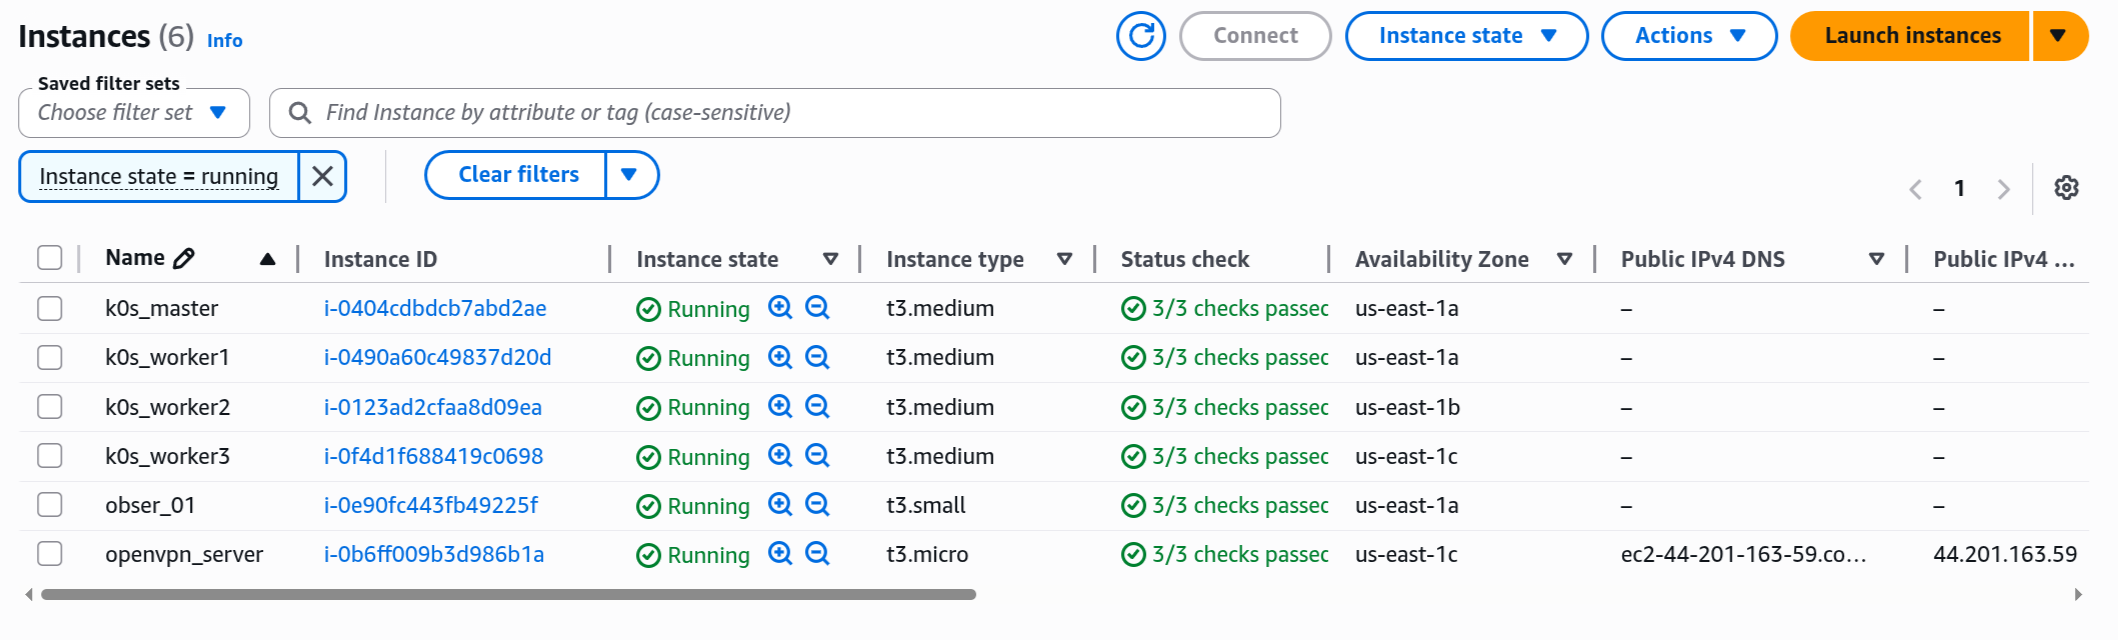
\includegraphics[width=1.0\textwidth]{graphics/chapter-5/5_1_infra/ec2.png}
    \captionof{figure}{Các máy ảo EC2 được Terraform khởi tạo và đưa về trạng thái hoạt động}
    \label{fig:terraform-ec2-running}
\end{center}

\noindent Hình \ref{fig:terraform-ec2-running} xác nhận các máy ảo chính của môi trường thực nghiệm đã được tạo và đi vào trạng thái \textit{Running}, bao gồm một node \texttt{k0s\_master}, ba worker \texttt{k0s\_worker1}, \texttt{k0s\_worker2}, \texttt{k0s\_worker3}, một máy chủ giám sát \texttt{observ\_01} và một máy \texttt{openvpn\_server}. Toàn bộ instance đều vượt qua \textit{status check}, đồng thời được phân bố trên các Availability Zone đúng theo thiết kế hạ tầng đã mô tả ở phần trước. Kết quả này cho thấy lớp cơ sở hạ tầng đã sẵn sàng để tiếp tục cấu hình cụm Kubernetes, công cụ giám sát và môi trường thí nghiệm cho bài toán self-healing.

\begin{center}
    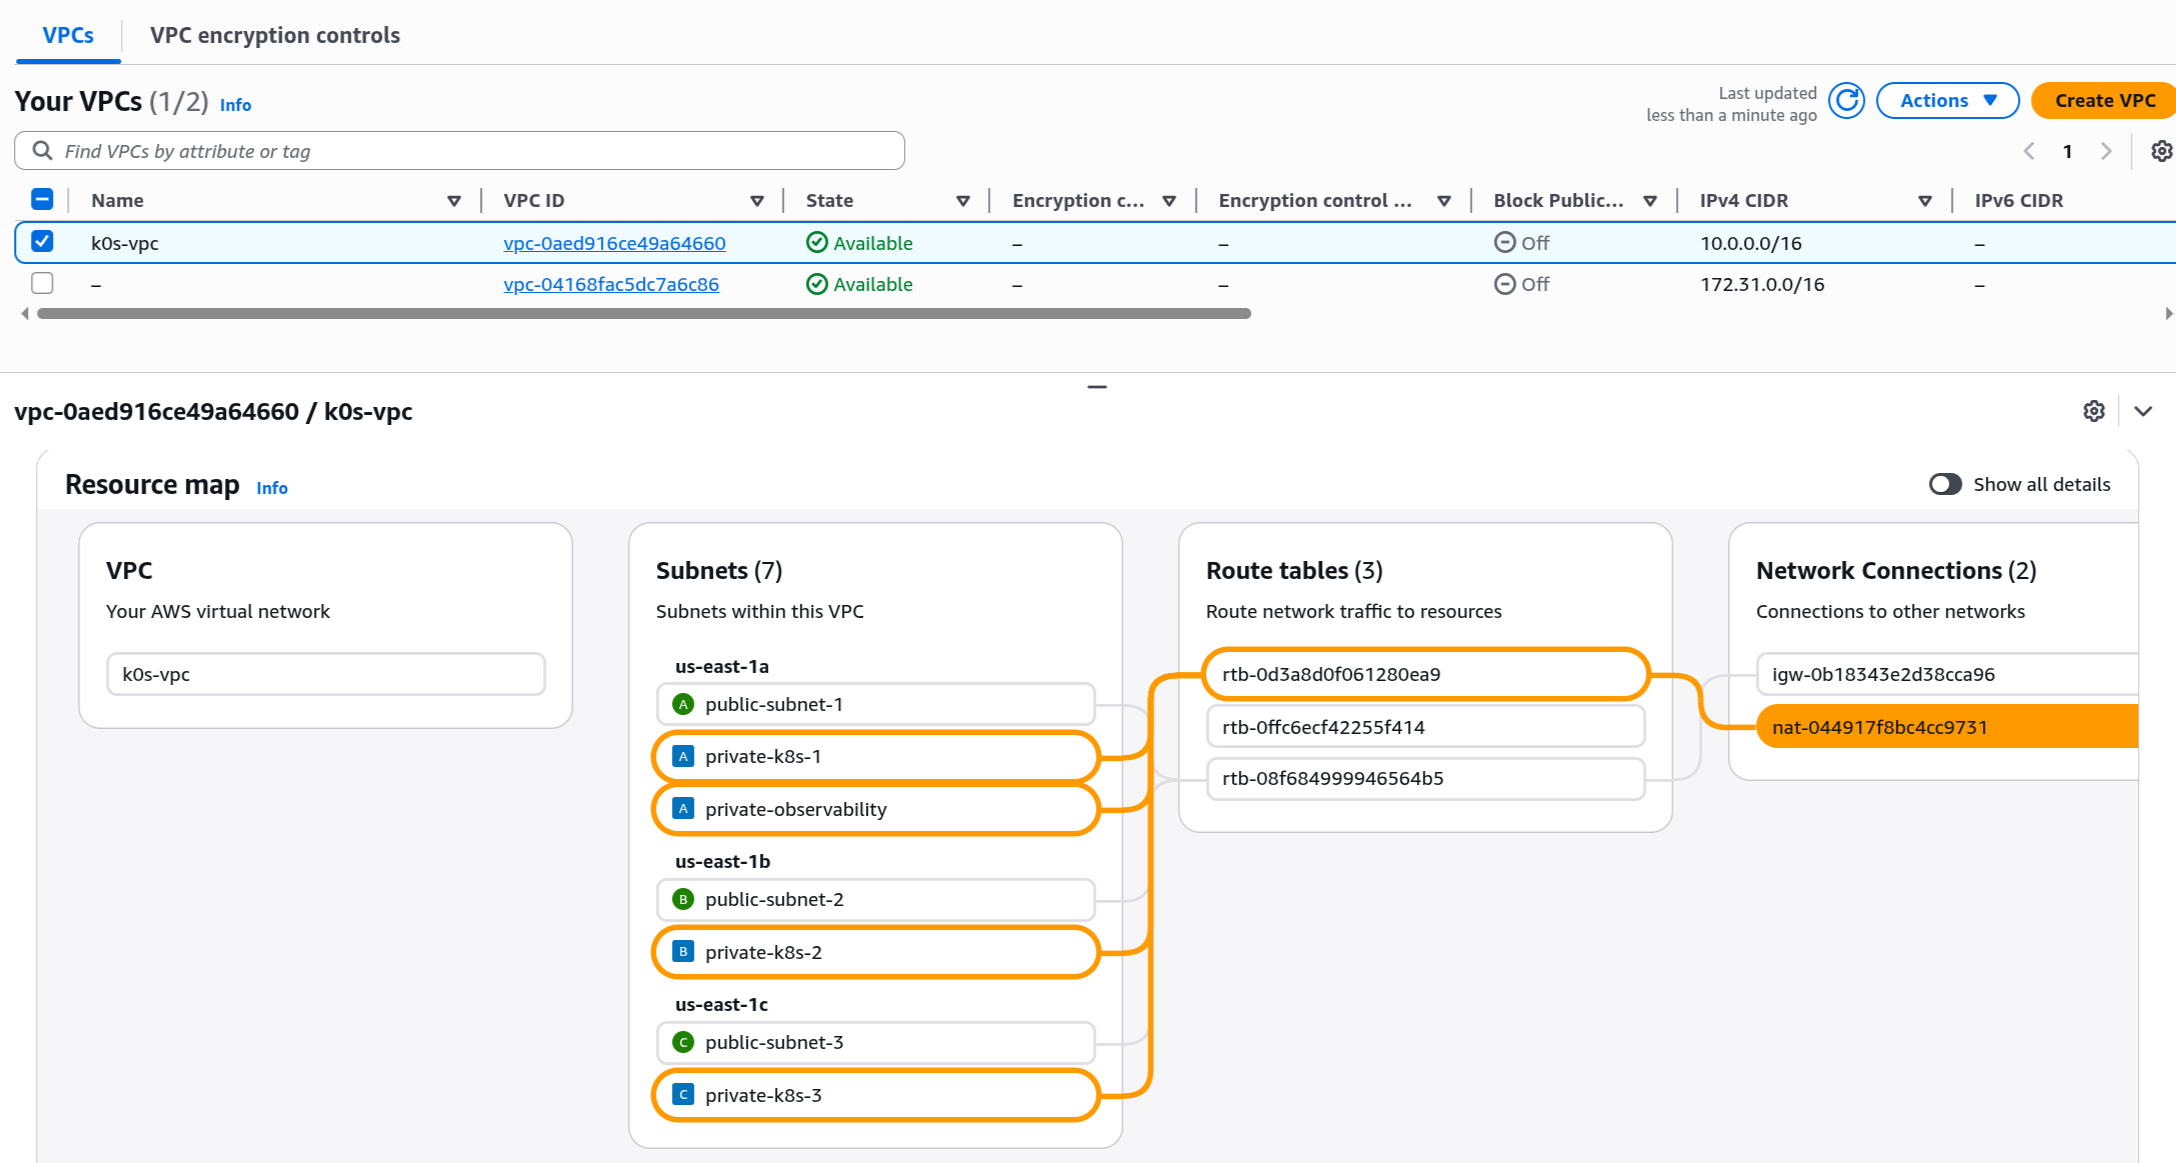
\includegraphics[width=1.0\textwidth]{graphics/chapter-5/5_1_infra/vpc.png}
    \captionof{figure}{Cấu trúc VPC và các subnet được Terraform khởi tạo trên AWS}
    \label{fig:terraform-vpc-topology}
\end{center}

\noindent Hình \ref{fig:terraform-vpc-topology} cho thấy Terraform đã khởi tạo thành công VPC với dải mạng 10.0.0.0/16, đồng thời phân tách rõ public subnet và private subnet trên ba Availability Zone.

\noindent Các subnet dành cho cụm Kubernetes gồm:
\begin{itemize}
    \item \texttt{private-k8s-1}
    \item \texttt{private-k8s-2}
    \item \texttt{private-k8s-3}
\end{itemize}
\noindent Trong khi đó, subnet \texttt{private-observability} 
được sử dụng cho Prometheus và Grafana. Việc định tuyến private subnet 
thông qua NAT Gateway giúp các máy nội bộ có thể truy cập ra ngoài khi 
cần cài đặt và cập nhật gói, nhưng vẫn giữ được nguyên tắc không phơi lộ 
trực tiếp ra Internet.

\section{Cấu hình các công cụ sử dụng Ansible}

Để tự động hóa cấu hình hệ điều hành và thiết lập phần mềm trên các máy chủ EC2 
đã được khởi tạo bởi Terraform, công cụ Ansible được sử dụng. Với kiến trúc 
không tác nhân (\textit{agentless}), Ansible thực hiện truyền tải các cấu hình 
thông qua kết nối SSH bảo mật, giúp thiết lập môi trường đồng bộ, nhất quán và giảm thiểu tối đa các thao tác quản trị thủ công. Các chỉ thị cấu hình được khai báo dưới dạng tệp tin YAML (\textit{Ansible Playbooks}).

\subsection{Cấu hình dịch vụ mạng riêng ảo sử dụng OpenVPN}

Dịch vụ OpenVPN Server được cấu hình và thiết lập tự động thông qua Ansible trên máy chủ đặt tại Public Subnet của AZ 3. Vai trò của thành phần này là thiết lập một đường truyền mã hóa bảo mật từ xa (VPN Tunnel) cho phép quản trị viên truy cập an toàn vào dải mạng nội bộ (Private Subnet) của VPC để thực hiện các thao tác quản trị cụm Kubernetes và hệ thống giám sát mà không cần công khai các cổng dịch vụ ra Internet.

Một phần cấu hình chính của OpenVPN được khai báo như sau:

\begin{lstlisting}
# OpenVPN basic
openvpn_port: 1194
openvpn_proto: udp

# VPN network
openvpn_network: 10.8.0.0
openvpn_netmask: 255.255.255.0
openvpn_tunnel_iface: tun0

# Directories
openvpn_server_dir: /etc/openvpn/server
easy_rsa_dir: /etc/openvpn/easy-rsa

# Client
openvpn_client_name: devops
openvpn_public_ip: "{{ ansible_host }}"

# EC2 private interface (AWS Ubuntu)
openvpn_private_iface: ens5

# ===== VPC ROUTE =====
# CIDR cua VPC PROD
vpc_network: 10.0.0.0
vpc_netmask: 255.255.0.0

# DNS for client
openvpn_dns:
  - 8.8.8.8
  - 1.1.1.1
\end{lstlisting}

\noindent Về mặt định tuyến, OpenVPN tạo một mạng tunnel riêng với dải \texttt{10.8.0.0/24} trên interface \texttt{tun0}. Khi máy khách kết nối vào VPN, lưu lượng quản trị sẽ đi trước hết vào tunnel này, sau đó được máy chủ OpenVPN chuyển tiếp sang card mạng private \texttt{ens5} để truy cập các tài nguyên nằm trong VPC nội bộ.

\noindent Cặp tham số \texttt{vpc\_network=10.0.0.0} và \texttt{vpc\_netmask=255.255.0.0} là phần quan trọng nhất của cấu hình routing, vì nó xác định đích đến cuối cùng của các gói tin từ phía client. Nói cách khác, OpenVPN phải biết rằng mọi lưu lượng hướng tới dải \texttt{10.0.0.0/16} cần được đẩy vào mạng VPC thay vì đi ra Internet công cộng. Nhờ đó, sau khi kết nối VPN, quản trị viên có thể truy cập các máy \texttt{k0s\_master}, \texttt{k0s\_worker*} và máy giám sát bằng địa chỉ private mà không cần mở cổng SSH trực tiếp ra ngoài.

\noindent Cách cấu hình này mang lại hai lợi ích chính. Thứ nhất, lớp quản trị được tách biệt khỏi luồng truy cập của người dùng cuối, giúp giảm bề mặt tấn công lên cụm thực nghiệm. Thứ hai, toàn bộ thao tác Ansible, SSH và kiểm tra dịch vụ nội bộ đều có thể thực hiện thông qua VPN, bảo đảm đúng nguyên tắc chỉ cho phép truy cập riêng tư vào các subnet vận hành Kubernetes và observability.

\subsection{Cấu hình cụm Kubernetes}

Quy trình thiết lập cụm Kubernetes được tự động hóa hoàn toàn bằng Ansible Playbook bao gồm các công đoạn chính:
\begin{itemize}
    \item \textbf{Chuẩn bị môi trường:} Tắt phân vùng swap, cấu hình các tham số nhân hệ điều hành (\textit{sysctl}) cho mạng container và cài đặt container runtime (như \texttt{containerd}).
    \item \textbf{Cấu hình Master Node:} Khởi tạo nút điều khiển (Control Plane), thiết lập tệp cấu hình \texttt{kubeconfig} và cài đặt Container Network Interface (CNI) để thiết lập mạng nội bộ cho các Pods.
    \item \textbf{Gia nhập các Worker Nodes:} Ansible tự động trích xuất mã thông báo gia nhập (\textit{join token}) từ Master Node và thực thi lệnh kết nối các Worker Nodes phân tán trên các AZs vào cụm.
\end{itemize}

\begin{center}
    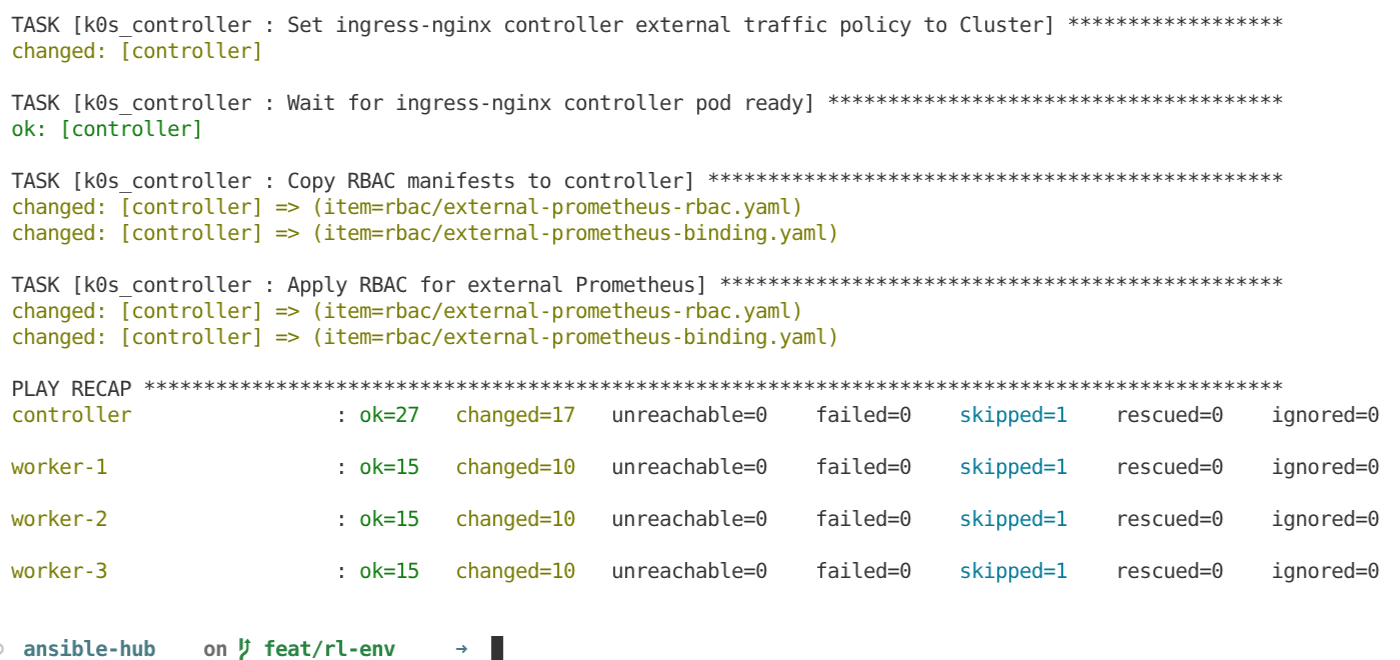
\includegraphics[width=1.0\textwidth]{graphics/chapter-5/5_2_kubernetes/config_k0s.png}
    \captionof{figure}{Kết quả chạy Ansible Playbook để cấu hình cụm k0s và RBAC cho Prometheus}
    \label{fig:k0s-ansible-config}
\end{center}

\noindent Hình \ref{fig:k0s-ansible-config} cho thấy quá trình Ansible thực thi các tác vụ cấu hình trên nút controller, bao gồm thiết lập ingress-nginx, chờ Pod sẵn sàng và áp dụng RBAC cho external Prometheus. Phần \texttt{PLAY RECAP} xác nhận toàn bộ các máy \texttt{controller}, \texttt{worker-1}, \texttt{worker-2} và \texttt{worker-3} đều hoàn tất không có lỗi, thể hiện việc triển khai cụm Kubernetes đã được tự động hóa ổn định và lặp lại được.

\begin{center}
    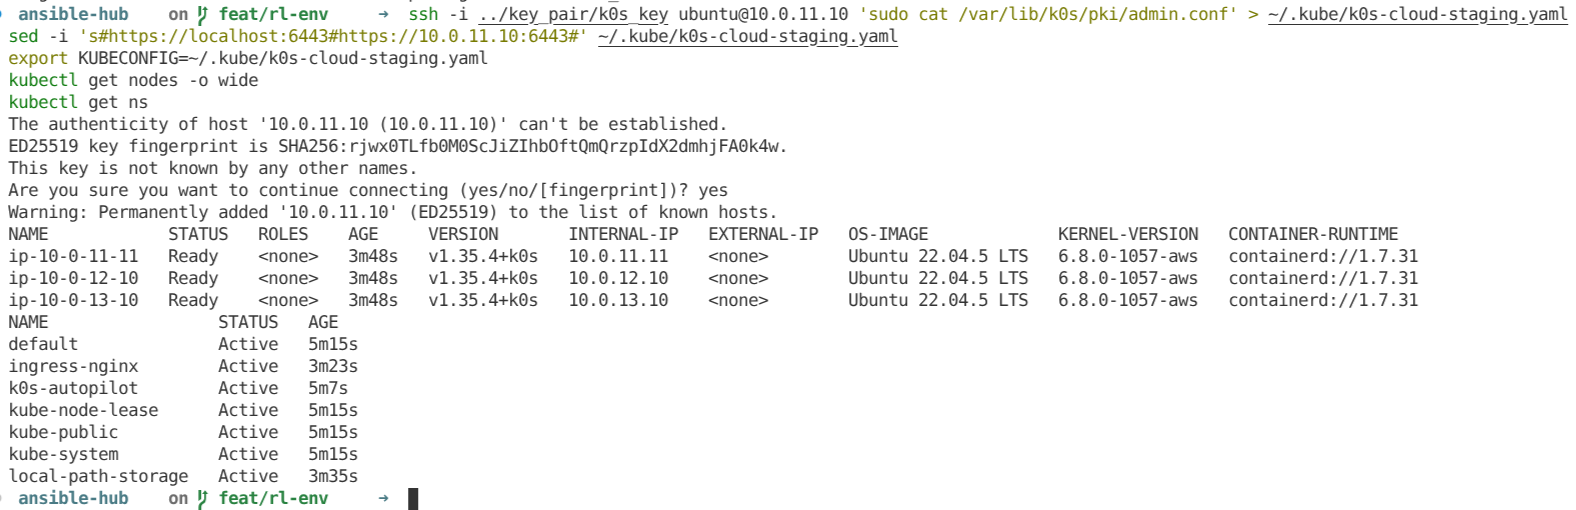
\includegraphics[width=1.0\textwidth]{graphics/chapter-5/5_2_kubernetes/connect_cluster.png}
    \captionof{figure}{Kết nối vào cụm k0s và kiểm tra trạng thái node, namespace sau triển khai}
    \label{fig:k0s-cluster-connect}
\end{center}

\noindent Từ Hình \ref{fig:k0s-cluster-connect}, có thể thấy tệp \texttt{kubeconfig} được trích xuất từ controller và hiệu chỉnh để truy cập qua địa chỉ private \texttt{10.0.11.10:6443}. Kết quả \texttt{kubectl get nodes -o wide} xác nhận ba worker node đã ở trạng thái \texttt{Ready}, đồng thời các namespace hệ thống như \texttt{default}, \texttt{kube-system}, \texttt{ingress-nginx} và \texttt{local-path-storage} đều ở trạng thái \texttt{Active}. Điều này cho thấy cụm Kubernetes đã sẵn sàng làm nền tảng triển khai microservices, giám sát và tác nhân RL ở các bước tiếp theo.

\subsection{Cấu hình hệ thống giám sát sử dụng Prometheus và Grafana}

Hệ thống giám sát được cấu hình tập trung trên máy chủ chuyên dụng đặt tại Private Subnet của AZ 1 nhằm đảm bảo tính toàn vẹn dữ liệu:
\begin{itemize}
    \item \textbf{Prometheus:} Được cấu hình thông qua Ansible để tự động phát hiện dịch vụ (\textit{service discovery}) trong cụm Kubernetes, thu thập dữ liệu metrics từ \texttt{node-exporter} (được Ansible cài đặt trên từng node) và \texttt{kube-state-metrics} theo chu kỳ 5 giây.
    \item \textbf{Grafana:} Được cấu hình sẵn các nguồn dữ liệu (\textit{Data Sources}) kết nối trực tiếp tới Prometheus và tự động nạp các bảng giao diện trực quan hóa (\textit{Dashboards}) để theo dõi hiệu năng tài nguyên hệ thống (CPU, RAM, Network) theo thời gian thực.
\end{itemize}

\begin{center}
    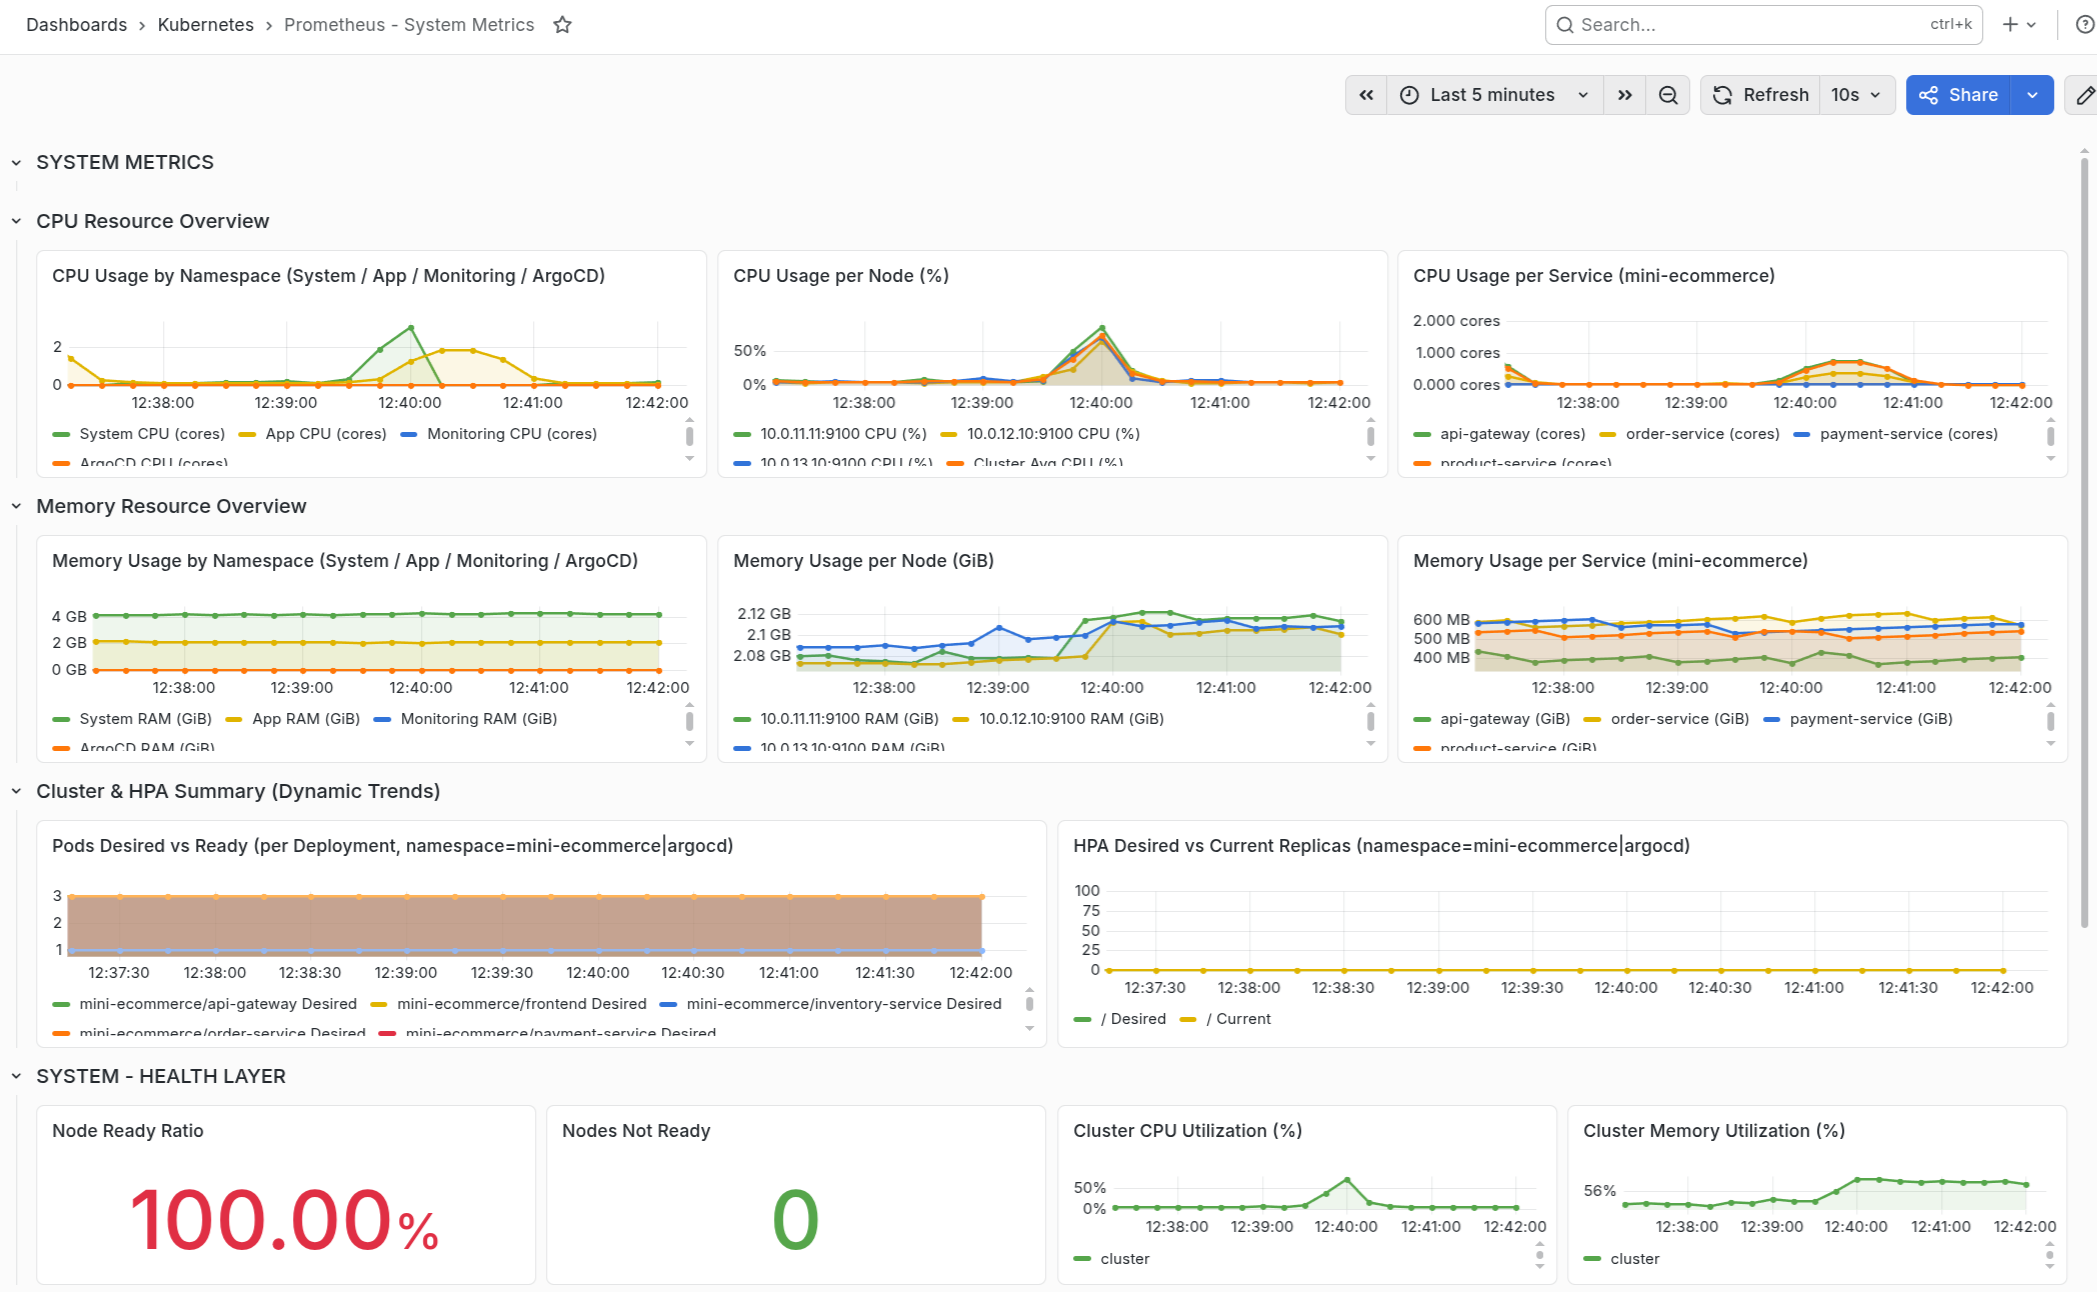
\includegraphics[width=1.0\textwidth]{graphics/chapter-5/5_3_monitoring/grafama_dashboard.png}
    \captionof{figure}{Dashboard Grafana theo dõi tài nguyên hệ thống và trạng thái dịch vụ}
    \label{fig:grafana-monitoring-dashboard}
\end{center}

\noindent Hình \ref{fig:grafana-monitoring-dashboard} cho thấy giao diện dashboard Grafana sau khi kết nối trực tiếp tới Prometheus. Các biểu đồ được tổ chức để theo dõi đồng thời tài nguyên hạ tầng, trạng thái Pod, độ trễ và các chỉ số phục vụ phân tích self-healing. Đây cũng là lớp quan sát trực quan giúp đối chiếu nhanh giữa thời điểm xảy ra sự cố, phản ứng của hệ thống và dữ liệu được xuất ra cho bước huấn luyện RL.

\section{Triển khai ứng dụng Microservices}

\subsection{Tổng quan ứng dụng}

Ứng dụng được sử dụng trong đồ án là hệ thống \textit{Mini Ecommerce Microservices} do tác giả tự phát triển, được xây dựng theo kiến trúc microservices đa ngôn ngữ nhằm phục vụ đồng thời cho thực nghiệm DevOps, observability và học tăng cường. Hệ thống mô phỏng một quy trình thương mại điện tử thu gọn, trong đó người dùng có thể đăng nhập, xem sản phẩm, kiểm tra tồn kho và tạo đơn hàng thông qua một điểm vào duy nhất là \texttt{api-gateway}.

\begin{center}
    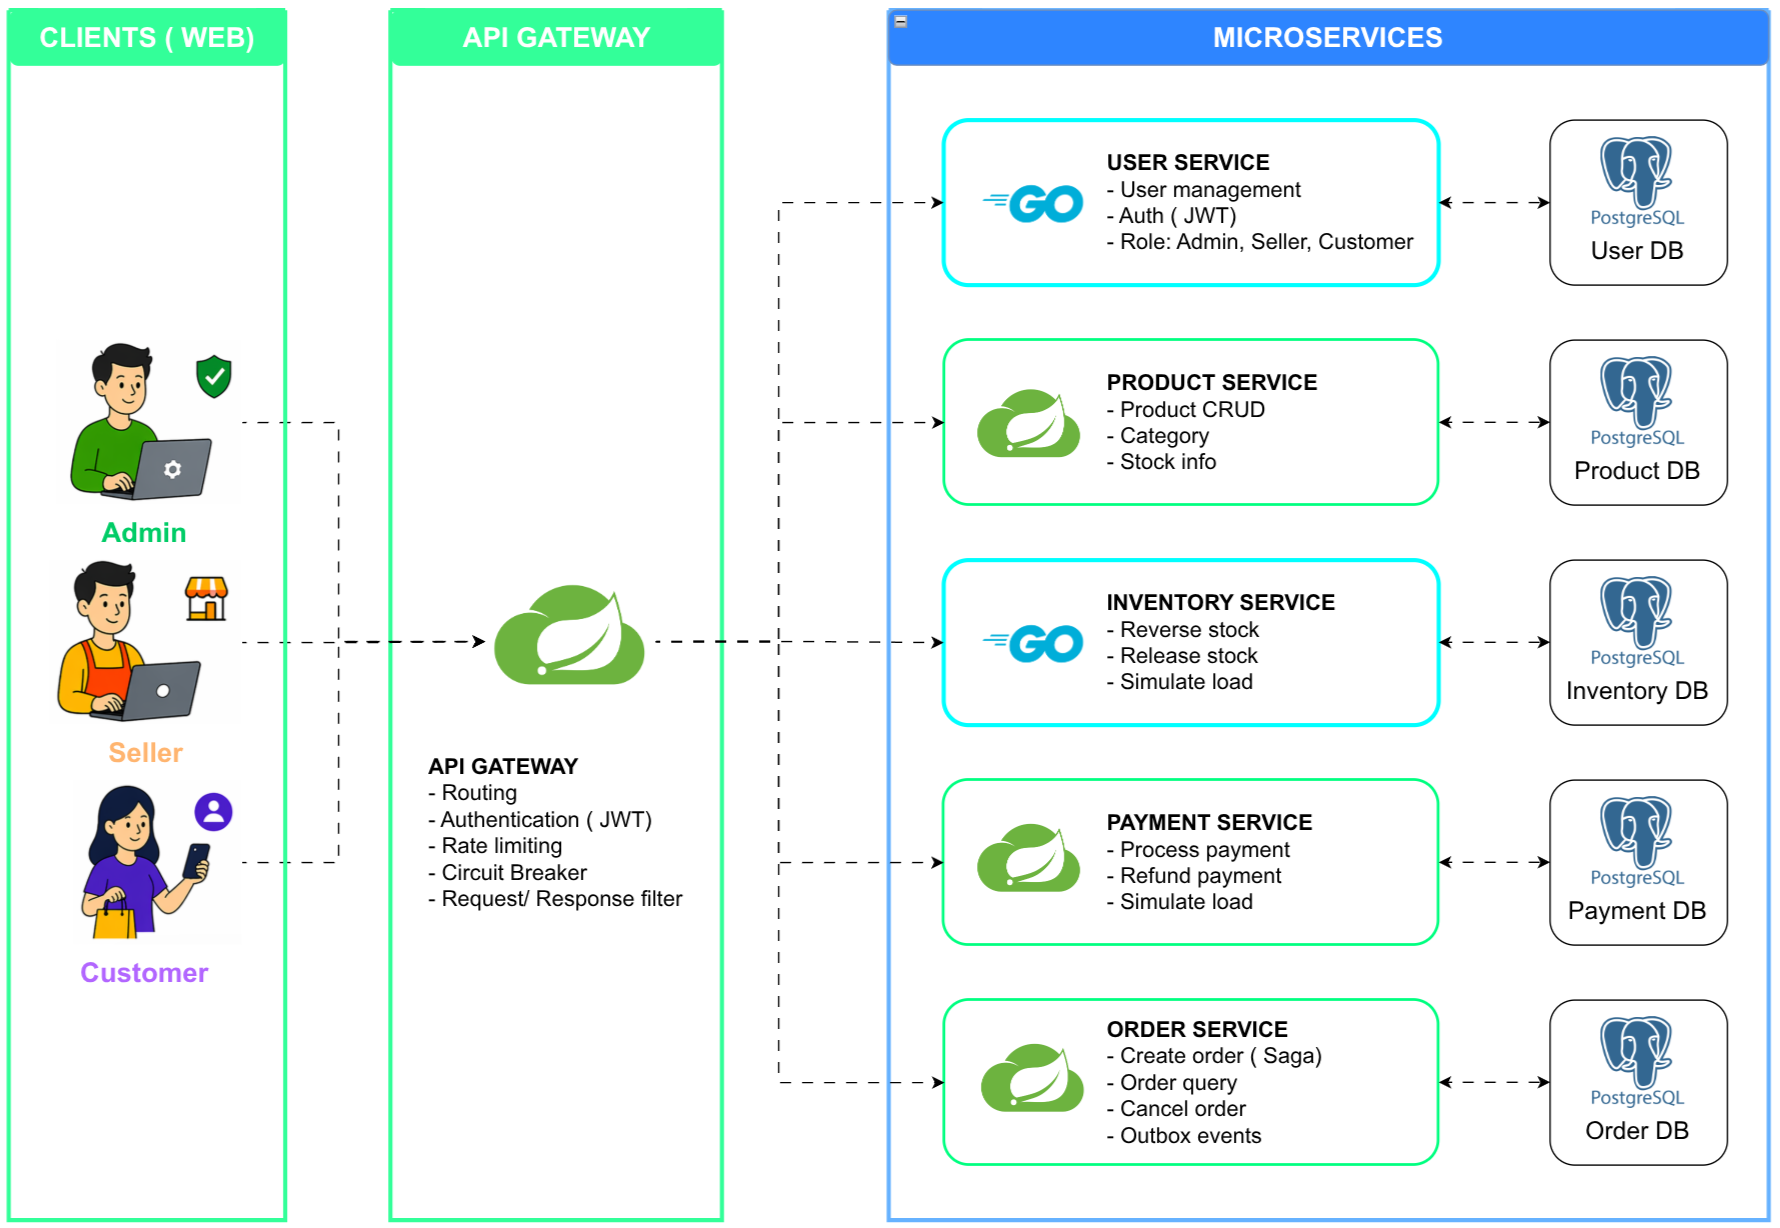
\includegraphics[width=0.97\textwidth]{graphics/chapter-5/5_4_application/architecture.png}
    \captionof{figure}{Kiến trúc tổng quan của ứng dụng Mini Ecommerce Microservices}
    \label{fig:mini-ecommerce-architecture}
\end{center}

\noindent Hình \ref{fig:mini-ecommerce-architecture} minh họa luồng truy cập từ phía người dùng qua \texttt{api-gateway} tới các microservice nghiệp vụ và cơ sở dữ liệu tương ứng. Kiến trúc này thể hiện rõ vai trò của gateway như lớp định tuyến và kiểm soát truy cập tập trung, trong khi các service phía sau được tách biệt theo miền chức năng để bảo đảm tính độc lập khi triển khai, giám sát và phục hồi.

\begin{center}
    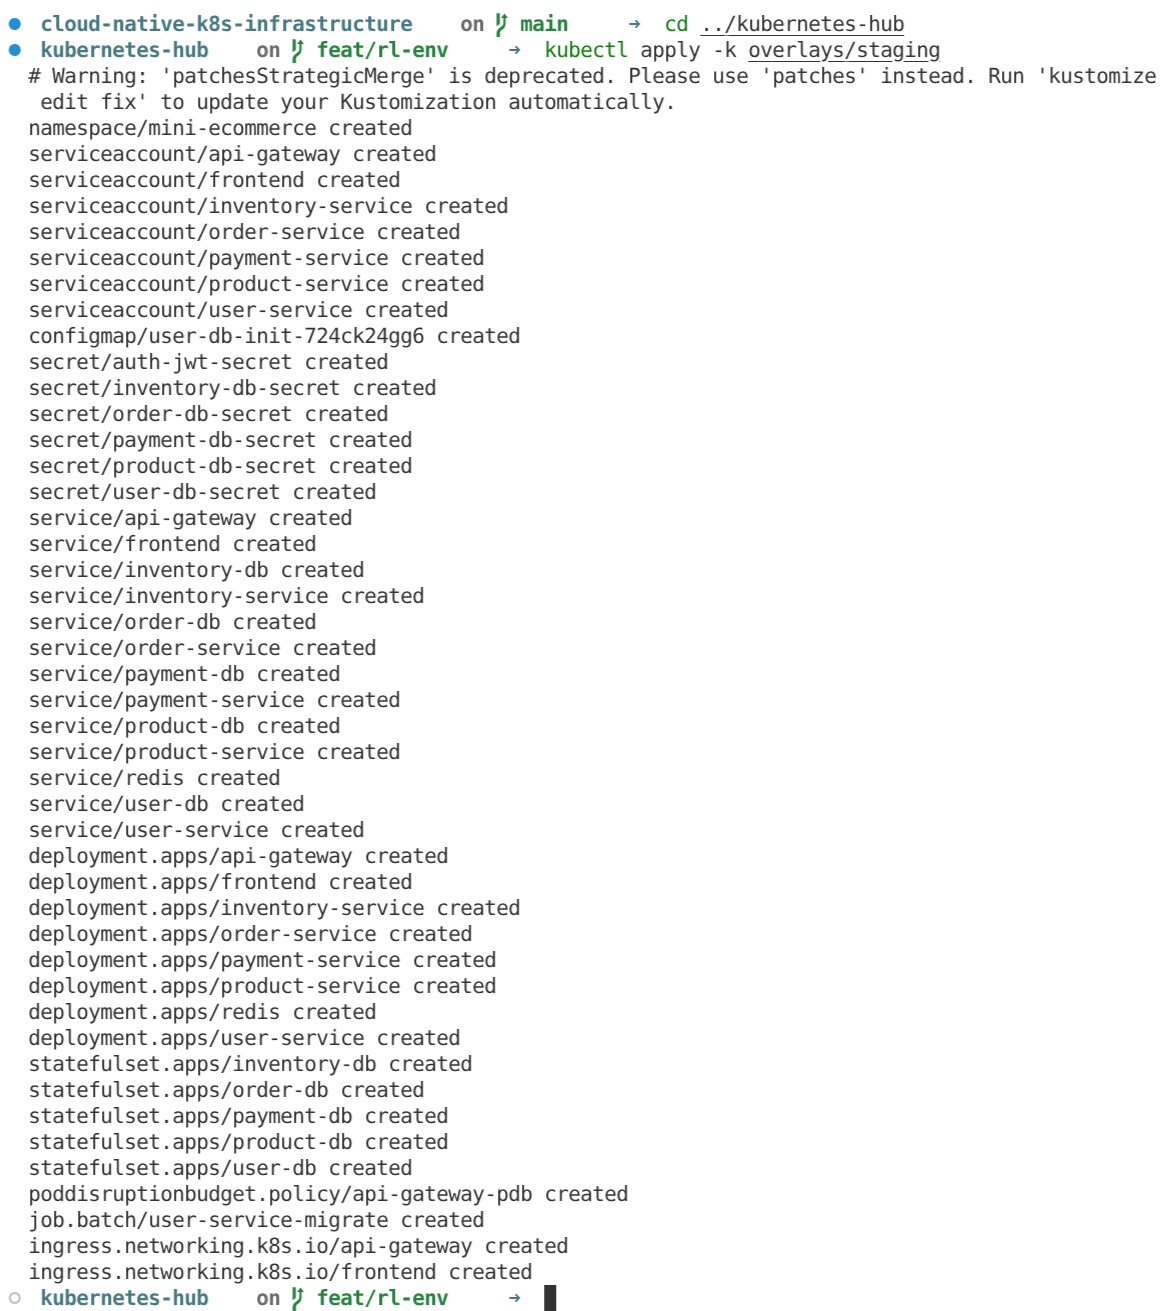
\includegraphics[width=0.95\textwidth]{graphics/chapter-5/5_4_application/deploy.png}
    \captionof{figure}{Triển khai bộ manifest ứng dụng microservices lên namespace \texttt{mini-ecommerce}}
    \label{fig:mini-ecommerce-deploy}
\end{center}

\noindent Ở mức triển khai, toàn bộ thành phần ứng dụng được đóng gói dưới dạng manifest Kubernetes và áp dụng bằng \texttt{kustomize} cho môi trường \texttt{staging}. Hình \ref{fig:mini-ecommerce-deploy} cho thấy quá trình \texttt{kubectl apply -k overlays/staging} đã khởi tạo đầy đủ namespace, service account, secret, service, deployment, statefulset, job migrate và ingress cần thiết. Cách tổ chức này giúp việc triển khai ứng dụng bám sát mô hình GitOps, đồng thời thuận tiện cho việc cập nhật cấu hình và tái lập thí nghiệm.

\begin{center}
    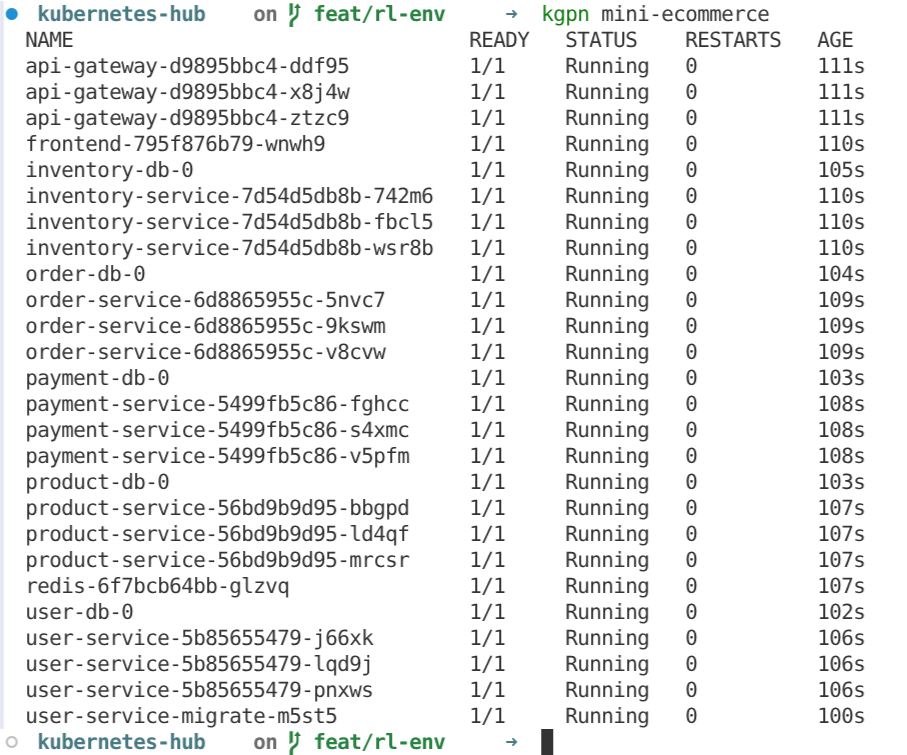
\includegraphics[width=0.7\textwidth]{graphics/chapter-5/5_4_application/get_pods.png}
    \captionof{figure}{Trạng thái Pod của ứng dụng sau khi triển khai lên Kubernetes}
    \label{fig:mini-ecommerce-pods}
\end{center}

\noindent Sau khi apply manifest, trạng thái runtime được kiểm tra nhanh bằng lệnh \texttt{kubectl get pods -n mini-ecommerce}. Hình \ref{fig:mini-ecommerce-pods} cho thấy các Pod của \texttt{api-gateway}, \texttt{frontend}, \texttt{user-service}, \texttt{product-service}, \texttt{inventory-service}, \texttt{payment-service}, \texttt{order-service}, \texttt{redis} và các cơ sở dữ liệu đều ở trạng thái \texttt{Running}. Đây là điều kiện cần để bước mô phỏng tải và mô phỏng sự cố ở các mục sau có thể diễn ra trên một môi trường dịch vụ hoàn chỉnh.

Về mặt thành phần, hệ thống runtime hiện tại gồm các dịch vụ chính:
\begin{itemize}
    \item \texttt{api-gateway}: điểm vào tập trung cho toàn bộ request từ phía người dùng.
    \item \texttt{user-service}: quản lý người dùng, xác thực và phân quyền.
    \item \texttt{product-service}: cung cấp chức năng quản lý và truy vấn sản phẩm.
    \item \texttt{inventory-service}: theo dõi, đặt giữ và hoàn trả tồn kho.
    \item \texttt{payment-service}: xử lý thanh toán và hoàn tiền khi cần bù trừ.
    \item \texttt{order-service}: điều phối quy trình tạo đơn hàng theo mô hình Saga.
    \item \texttt{front-end}: giao diện web phục vụ người dùng cuối.
    \item \texttt{Redis}: lớp trung gian bất đồng bộ cho trao đổi sự kiện giữa các service.
    \item \texttt{PostgreSQL}: hệ quản trị cơ sở dữ liệu được tách riêng theo từng miền nghiệp vụ.
\end{itemize}
\noindent Cách tổ chức này giúp hệ thống có đủ mức phân tán để quan sát các hiệu ứng lan truyền lỗi và hành vi phục hồi giữa nhiều thành phần.

\begin{center}
    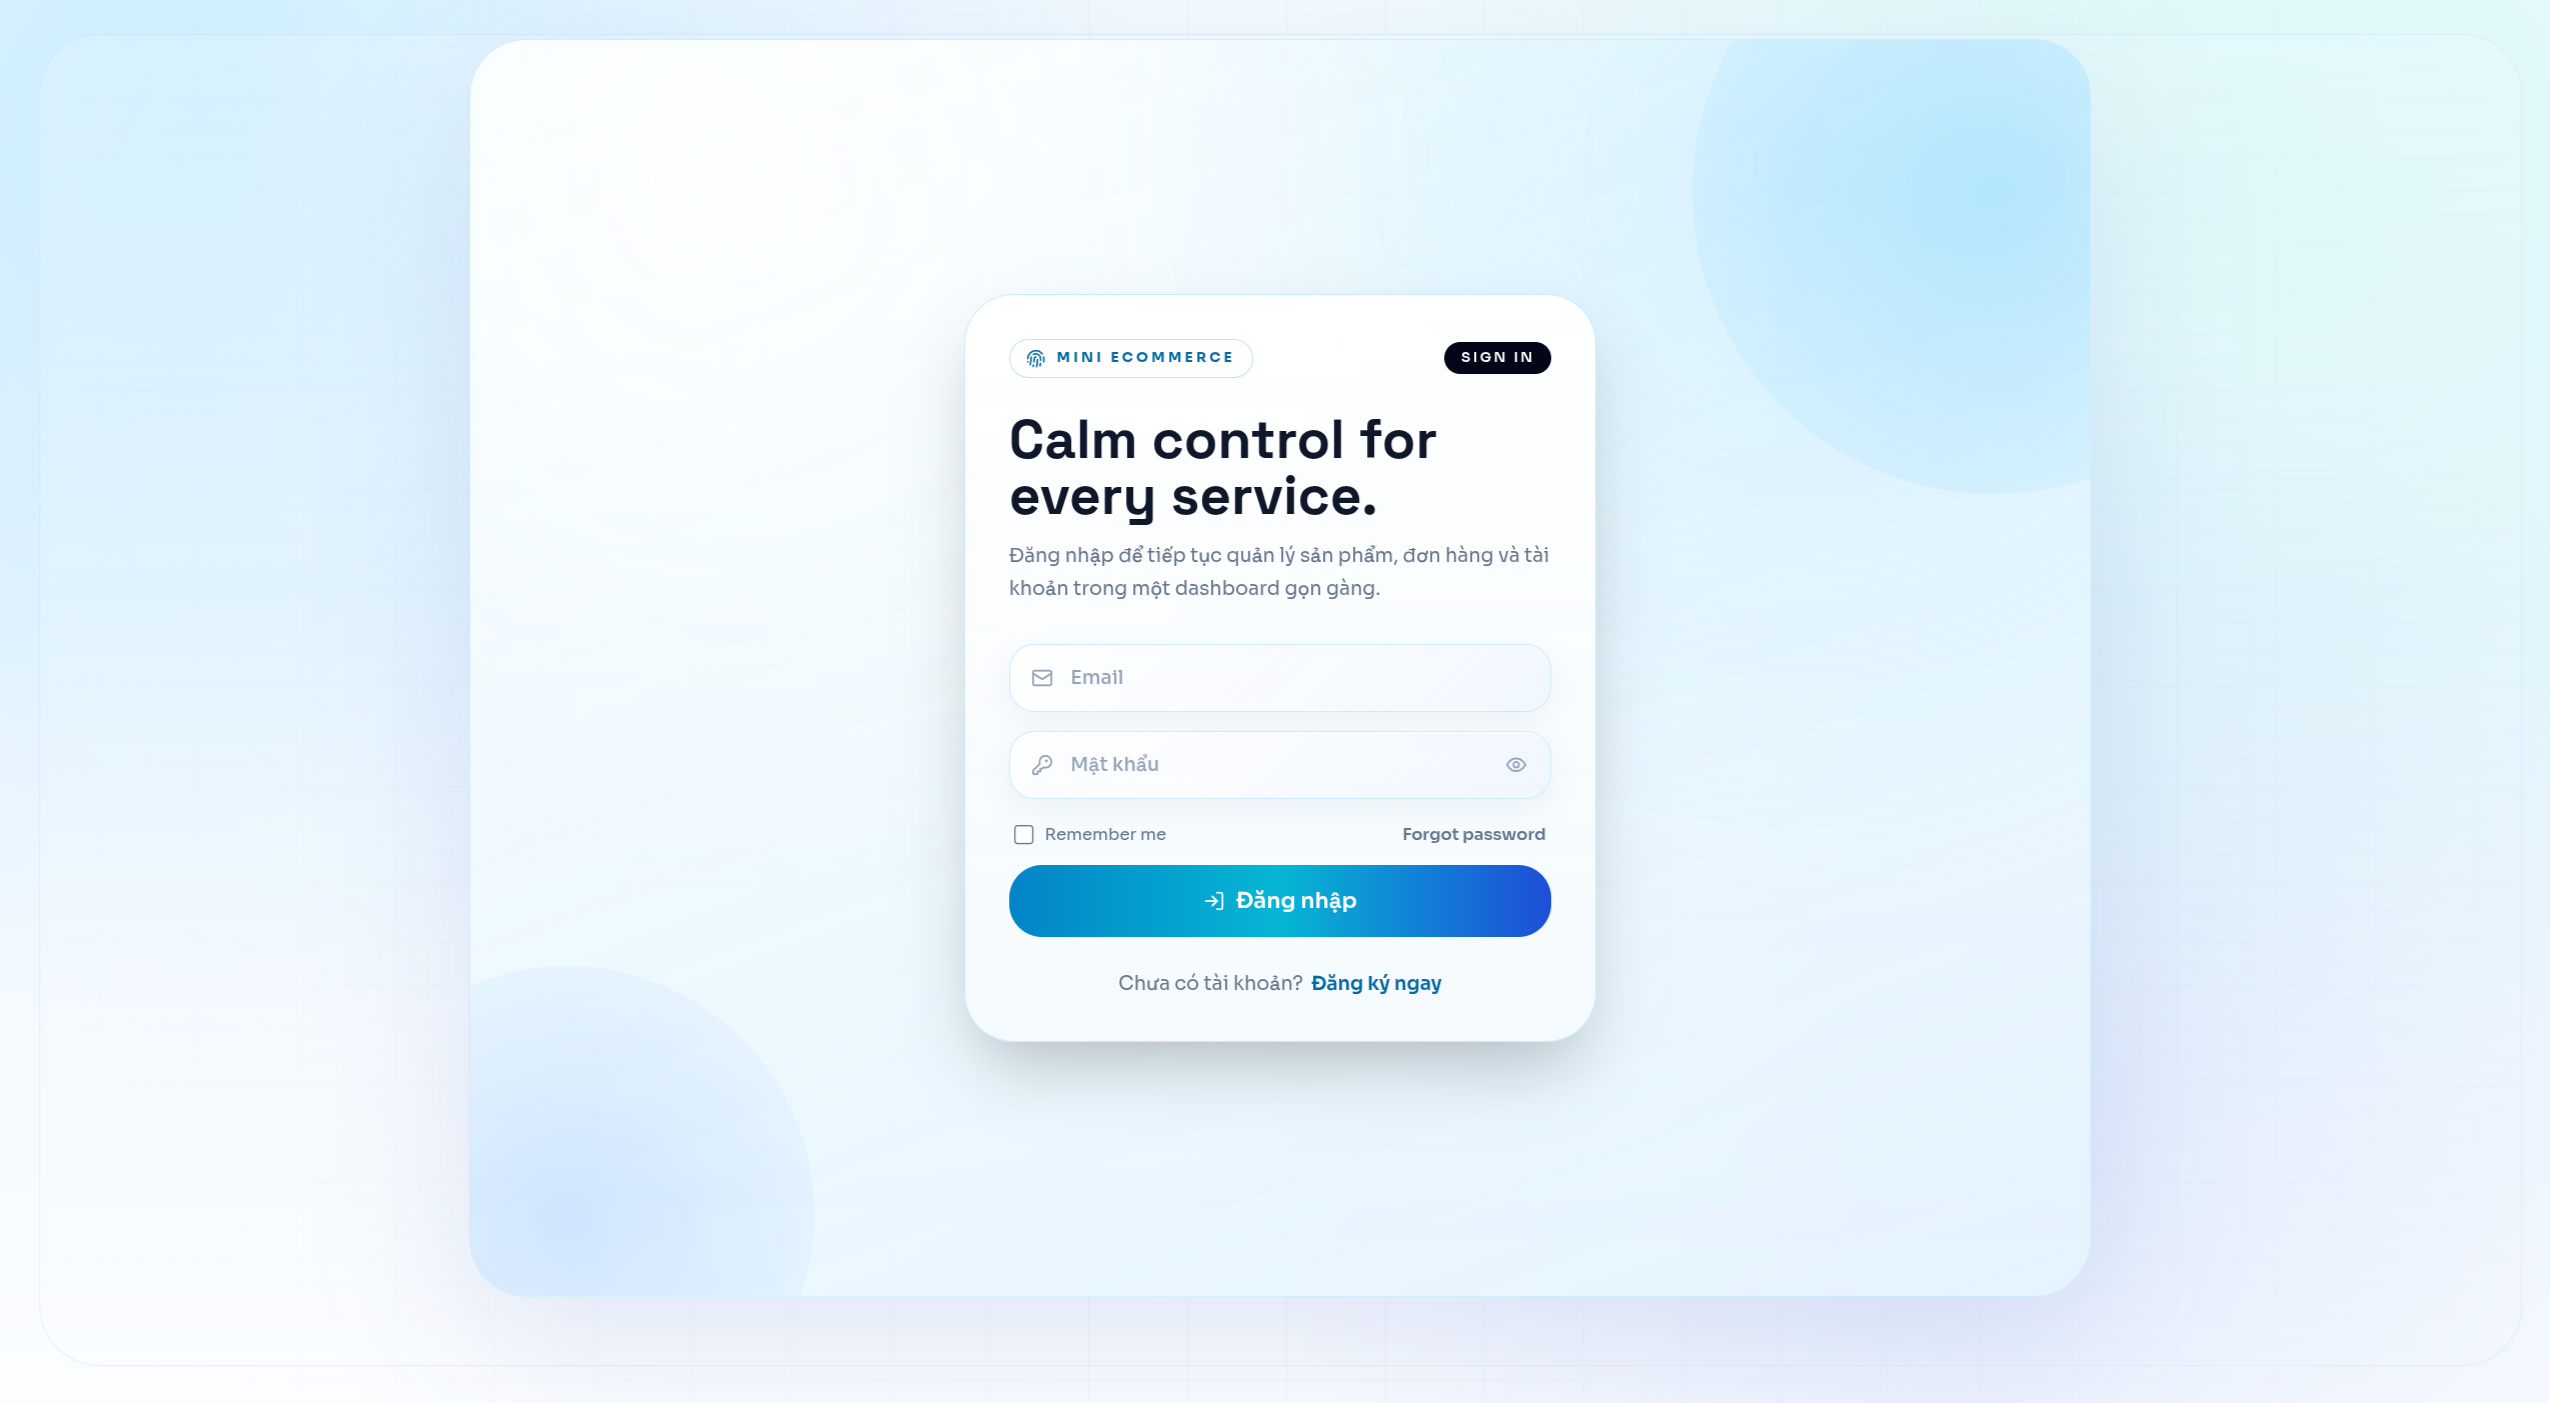
\includegraphics[width=0.98\textwidth]{graphics/chapter-5/5_4_application/login_register.png}
    \captionof{figure}{Giao diện đăng nhập của ứng dụng Mini Ecommerce}
    \label{fig:mini-ecommerce-login}
\end{center}

\noindent Ở phía người dùng cuối, ứng dụng cung cấp giao diện web để thao tác trực tiếp với các chức năng nghiệp vụ. Hình \ref{fig:mini-ecommerce-login} minh họa màn hình đăng nhập, nơi người dùng xác thực trước khi truy cập các chức năng quản trị sản phẩm, tồn kho và đơn hàng thông qua \texttt{api-gateway}.

\begin{center}
    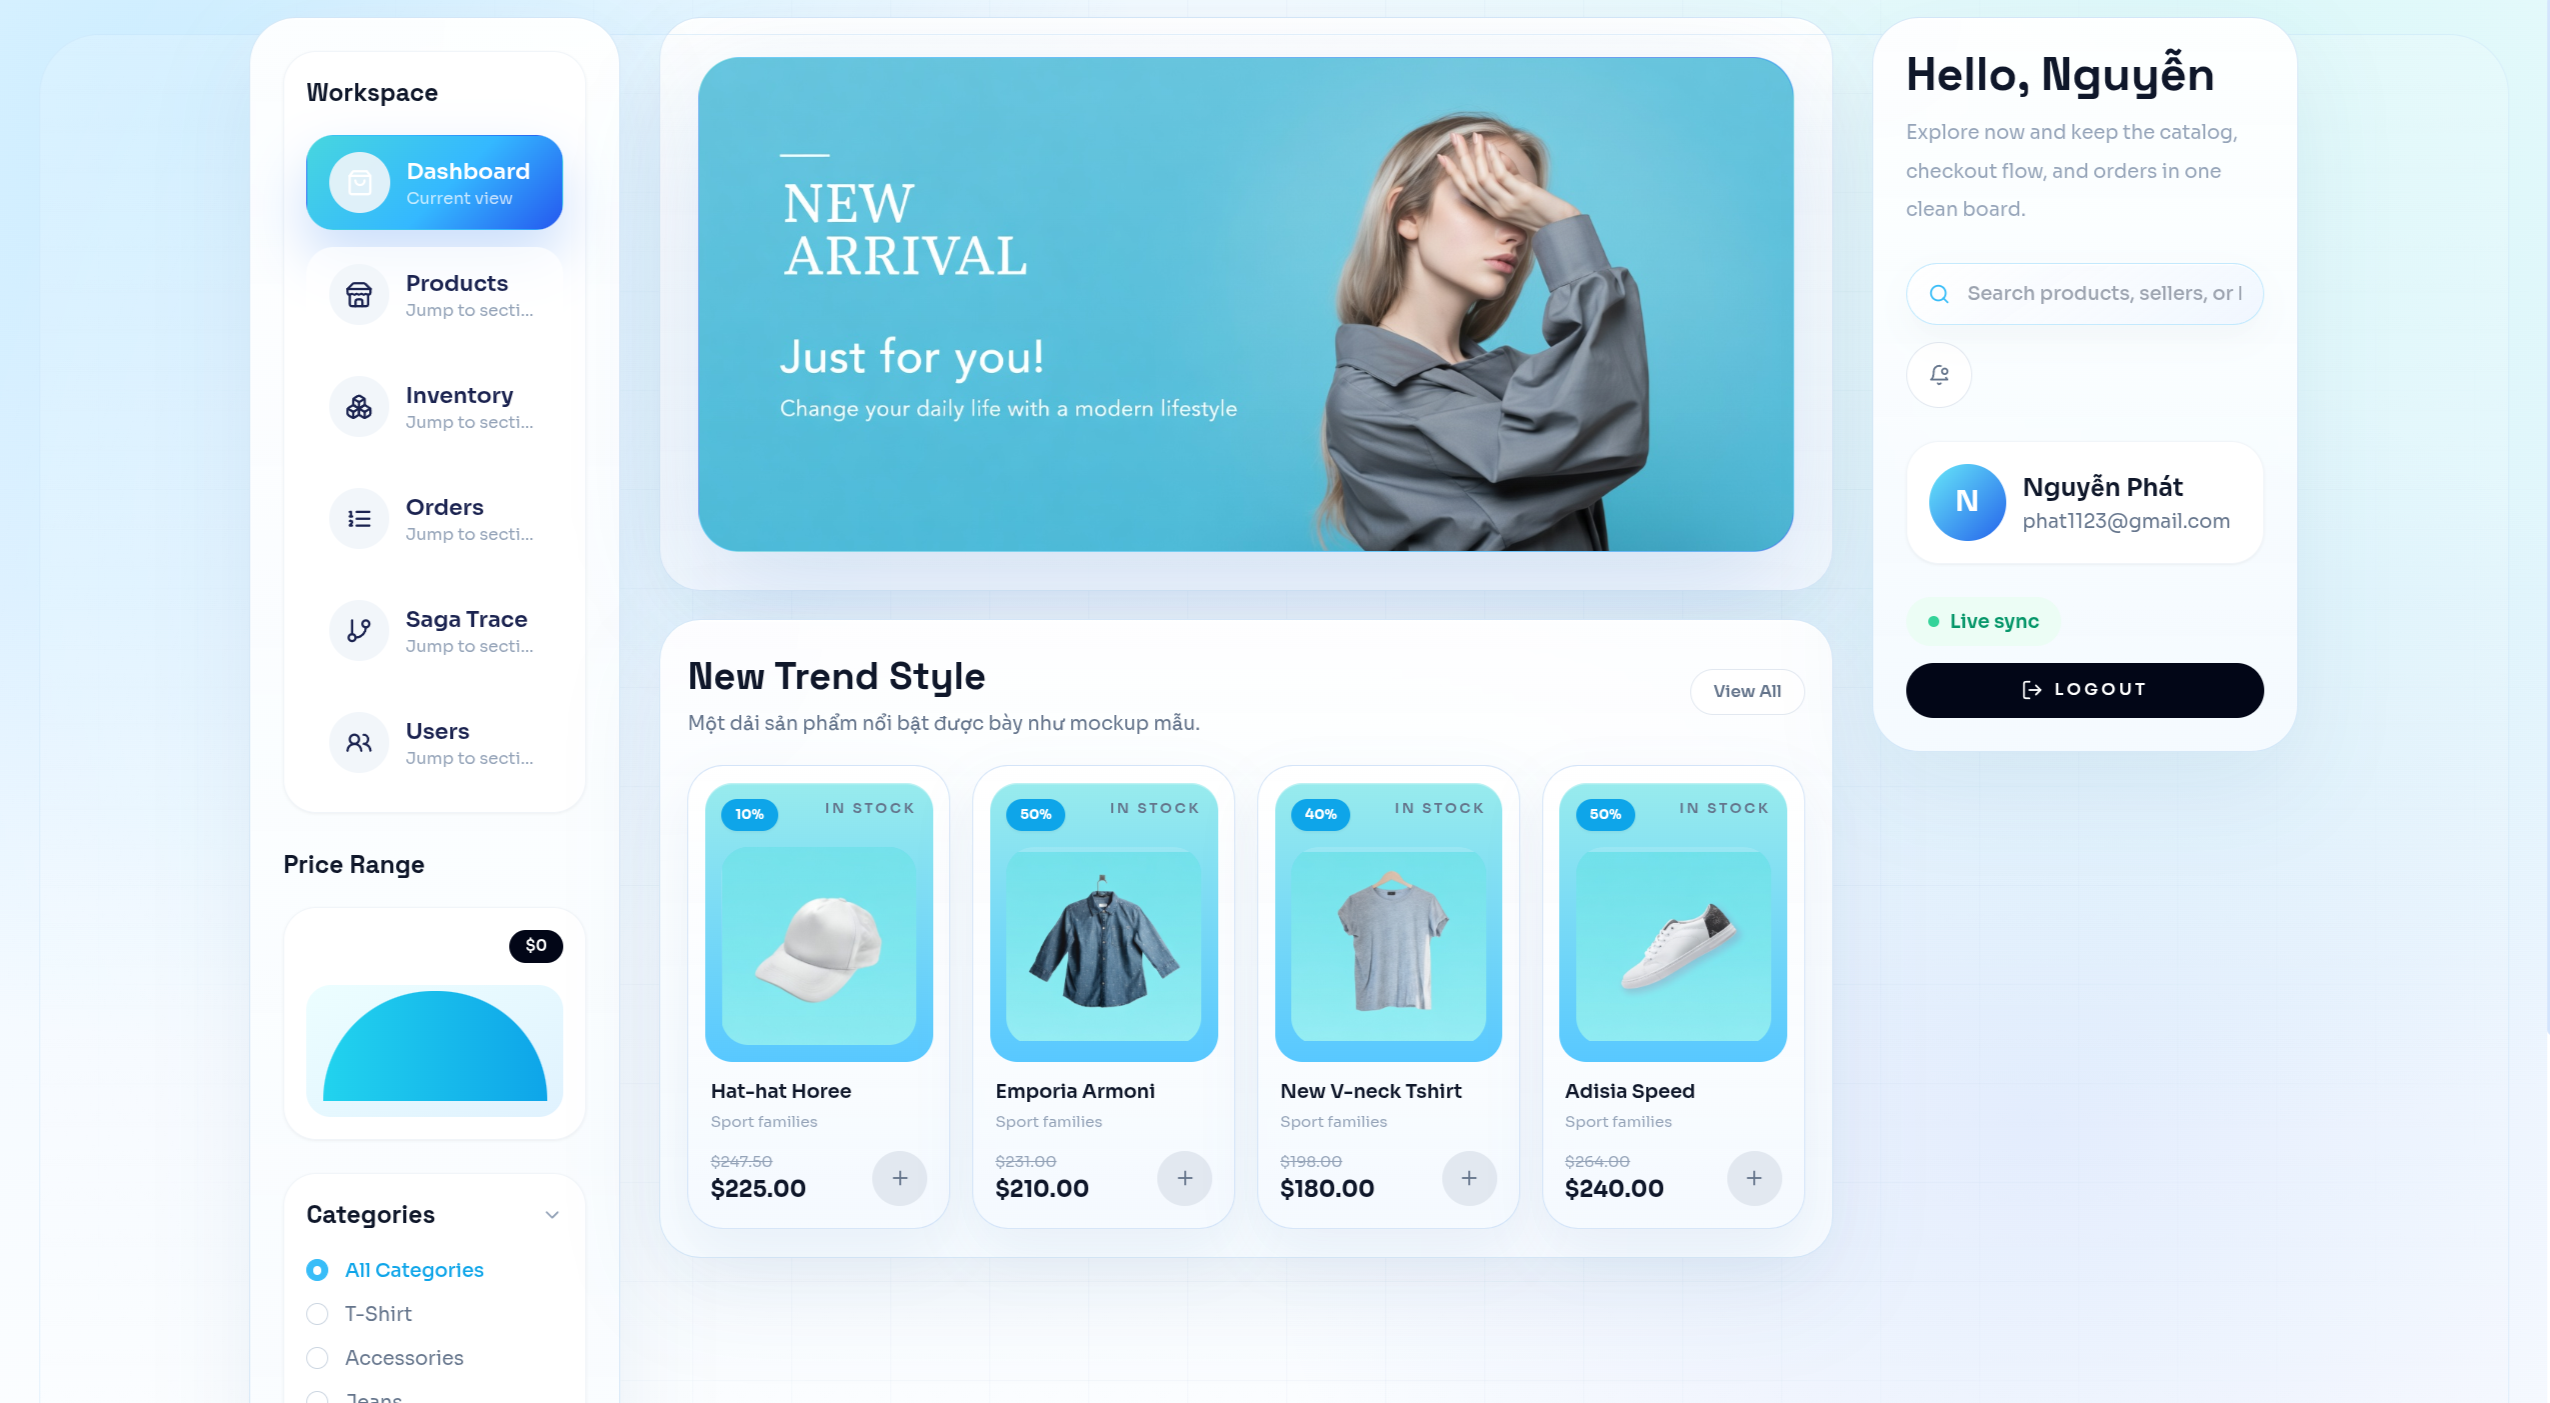
\includegraphics[width=0.98\textwidth]{graphics/chapter-5/5_4_application/main_ui.png}
    \captionof{figure}{Giao diện chính của hệ thống sau khi người dùng đăng nhập thành công}
    \label{fig:mini-ecommerce-main-ui}
\end{center}

\noindent Hình \ref{fig:mini-ecommerce-main-ui} cho thấy dashboard chính của ứng dụng với các khu vực chức năng như sản phẩm, tồn kho, đơn hàng, theo dõi saga và quản lý người dùng. Giao diện này là lớp tương tác trực tiếp để sinh ra các thao tác nghiệp vụ trong quá trình benchmark, từ đó tạo ra chuỗi request thực tế cho hệ thống microservices bên dưới.

Điểm quan trọng nhất của ứng dụng trong phạm vi đồ án là luồng xử lý đơn hàng theo mô hình \textit{Saga orchestration}. Khi một yêu cầu tạo đơn hàng được gửi tới \texttt{order-service}, hệ thống lần lượt thực hiện các bước đặt giữ tồn kho, xử lý thanh toán và cập nhật trạng thái đơn hàng; nếu một bước thất bại, cơ chế bù trừ sẽ được kích hoạt để hoàn tác các bước trước đó. Nhờ vậy, bài toán self-healing không chỉ dừng ở mức theo dõi tài nguyên hạ tầng mà còn gắn trực tiếp với chất lượng xử lý nghiệp vụ trong môi trường phân tán.

Ngoài các service nghiệp vụ, hệ thống còn tích hợp sẵn các thành phần giám sát được cài đặt cục bộ như \texttt{Prometheus}, \texttt{Grafana}, \texttt{Loki} và \texttt{Tempo}. Điều này tạo điều kiện thu thập đồng thời chỉ số hạ tầng, chỉ số ứng dụng và dấu vết truy vết phân tán, từ đó hình thành tập trạng thái đầu vào cho tác nhân RL. Vì vậy, \textit{Mini Ecommerce Microservices} vừa đóng vai trò hệ thống mục tiêu để triển khai self-healing, vừa là nguồn sinh dữ liệu thực nghiệm cho các bước huấn luyện và đánh giá ở các mục sau.

\section{Mô phỏng hoạt động thực tế của hệ thống}

\subsection{Mô phỏng lượng người dùng sử dụng K6}

Trong thực nghiệm, K6 được sử dụng để mô phỏng tải người dùng lên hệ thống \textit{mini-ecommerce} thông qua kịch bản \texttt{scripts-k6/user-journey.js}. Kịch bản bám theo luồng truy cập thực tế: đăng nhập, duyệt danh mục sản phẩm, xem chi tiết sản phẩm và truy vấn đơn hàng. Cách mô phỏng này giúp dữ liệu tải phản ánh sát hành vi nghiệp vụ thay vì chỉ gửi request tổng hợp.

Quá trình chạy được điều phối bởi script \texttt{scripts/run-user-journey.sh}. Script này tự động nạp cấu hình từ tệp môi trường, seed dữ liệu khách hàng/sản phẩm trước khi chạy (nếu bật), thực thi K6, sau đó dọn dẹp dữ liệu seed để tránh ảnh hưởng lần thử nghiệm kế tiếp. Nhờ đó, các lượt chạy có tính lặp lại cao và thuận tiện so sánh giữa nhiều kịch bản chaos.

\begin{center}
    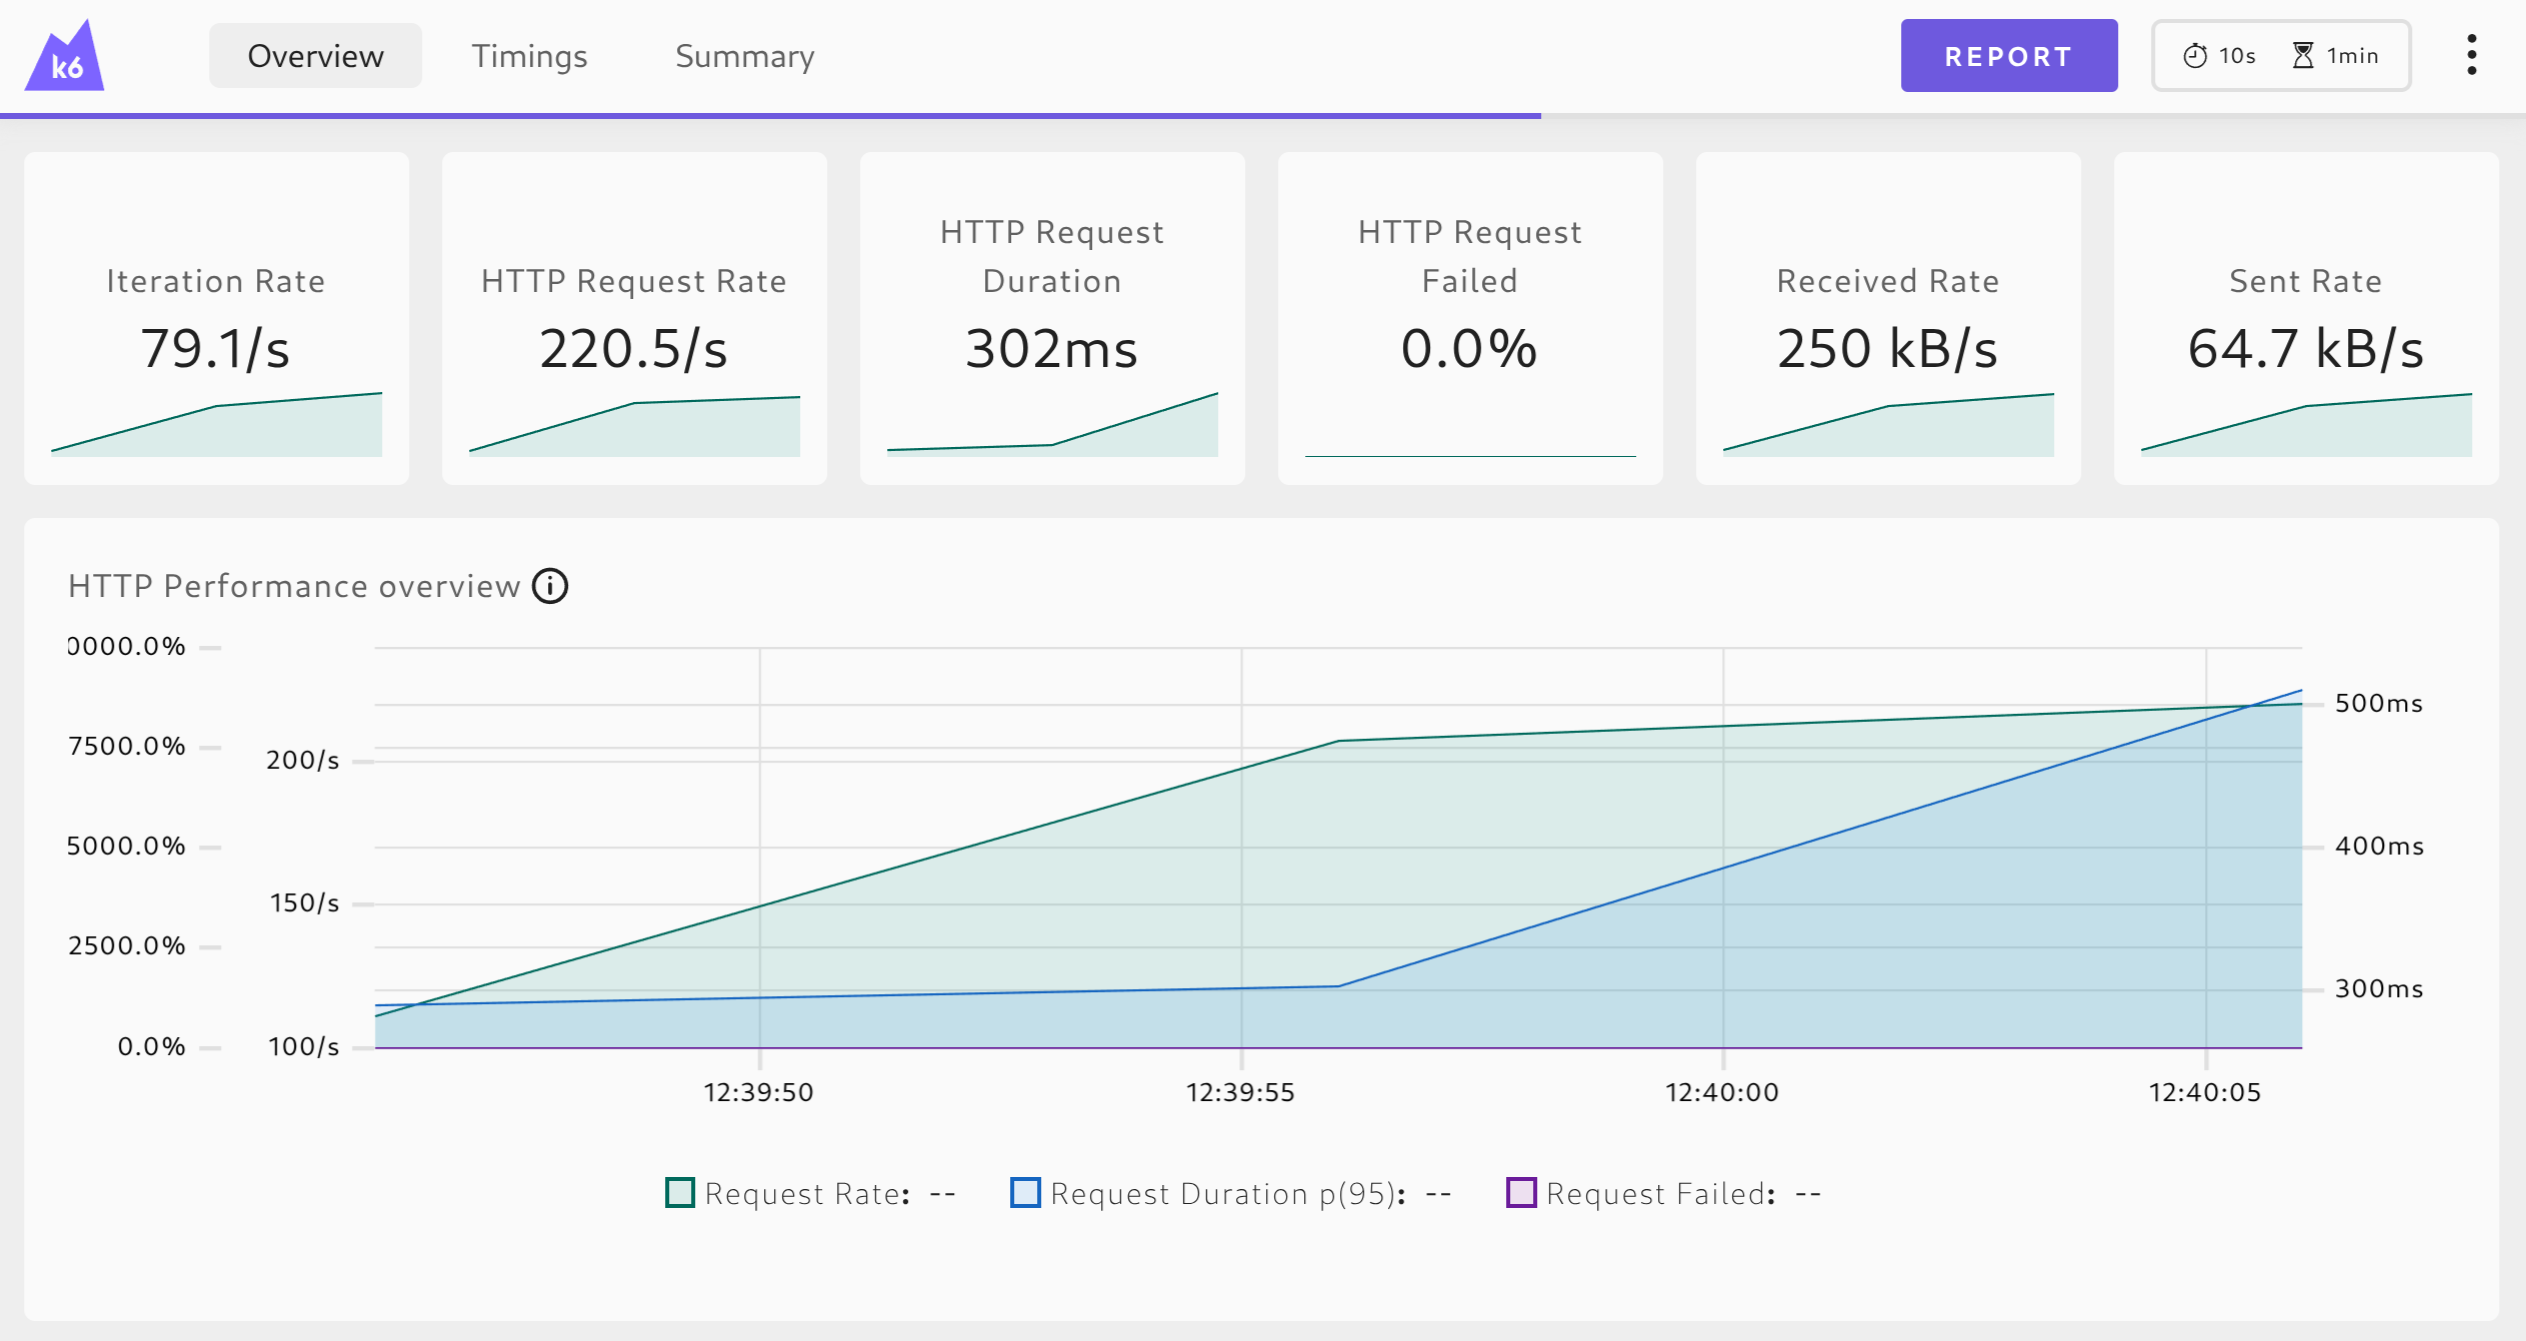
\includegraphics[width=0.98\textwidth]{graphics/chapter-5/5_5_k6/k6_overview.png}
    \captionof{figure}{Tổng quan dashboard K6 của một lượt chạy mô phỏng tải người dùng}
    \label{fig:k6-overview}
\end{center}

\noindent Hình \ref{fig:k6-overview} cho thấy dashboard tổng quan của K6 sau khi kết thúc một lượt benchmark. Các chỉ số ở phần đầu màn hình phản ánh mức tải quan sát được trong lượt chạy, gồm \textit{iteration rate}, \textit{HTTP request rate}, độ trễ HTTP và tỷ lệ request thất bại. Ở hình này, hệ thống vẫn duy trì \texttt{0.0\%} request lỗi trong khi thông lượng và độ trễ đã bắt đầu tăng theo mức tải.

\begin{center}
    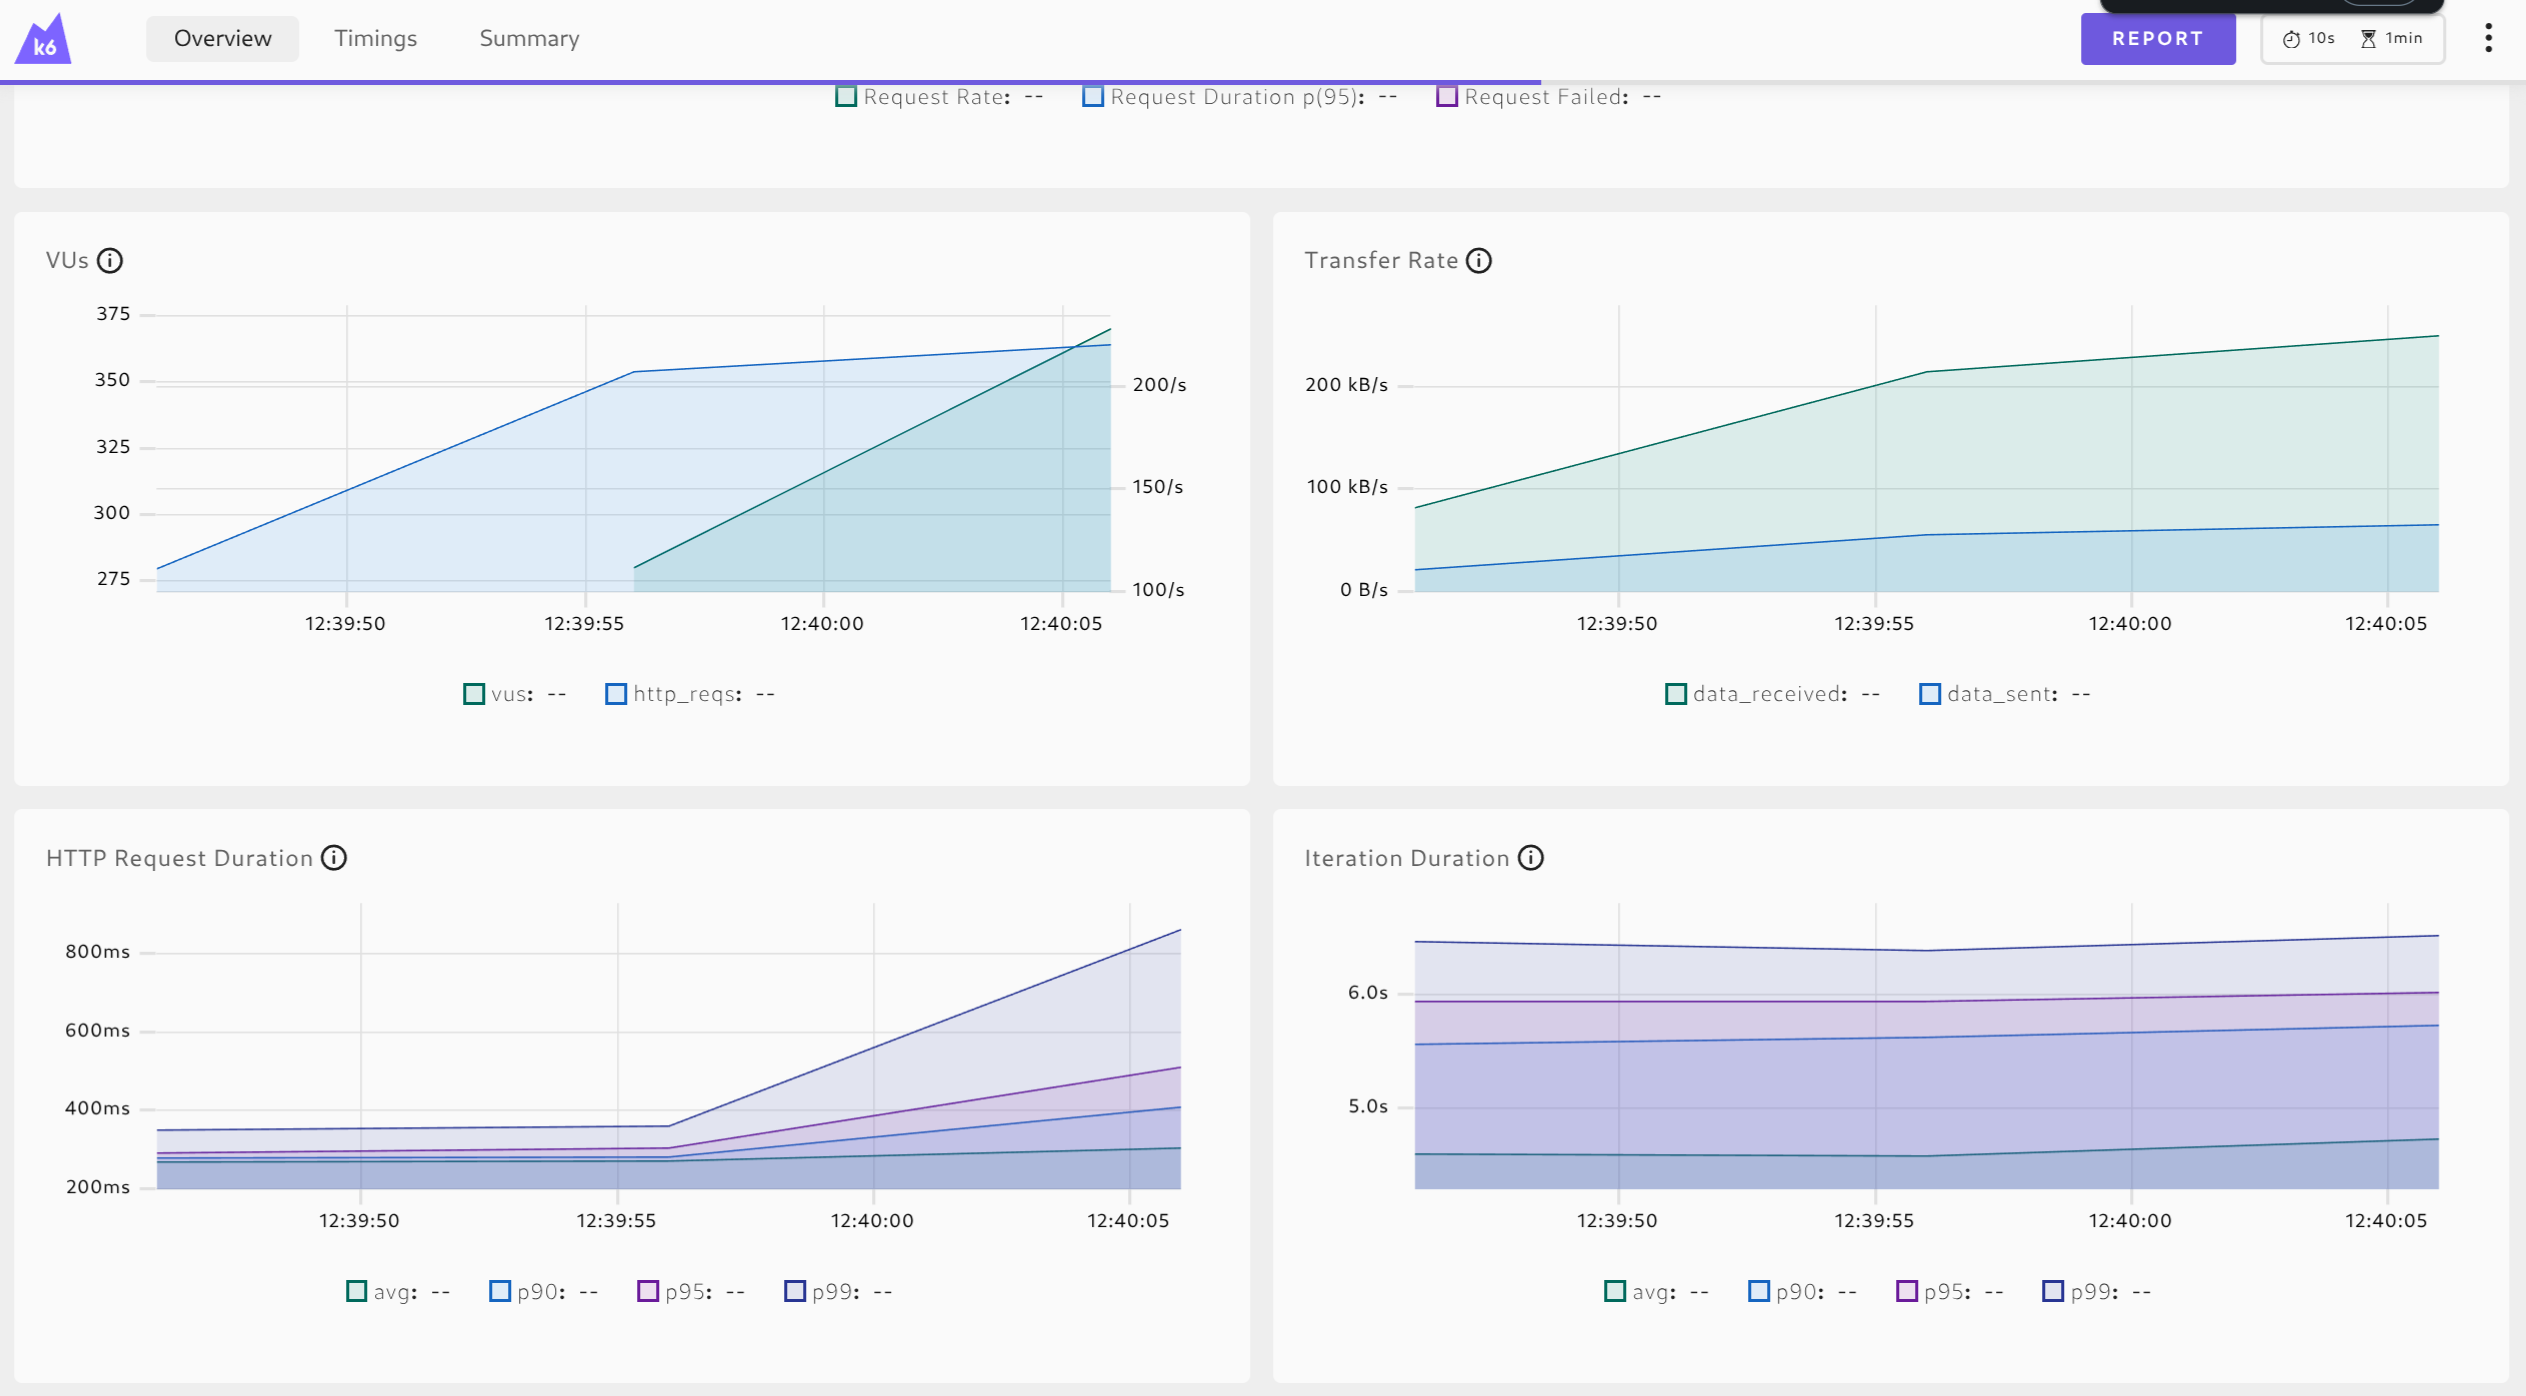
\includegraphics[width=0.98\textwidth]{graphics/chapter-5/5_5_k6/k6_performance_charts.png}
    \captionof{figure}{Biểu đồ tải, thông lượng và độ trễ trong lượt chạy K6}
    \label{fig:k6-performance-charts}
\end{center}

\noindent Hình \ref{fig:k6-performance-charts} thể hiện rõ quá trình tăng tải theo từng bước. Số lượng \textit{virtual users} tăng dần kéo theo \textit{HTTP request rate} và \textit{transfer rate} tăng tương ứng, trong khi độ trễ \textit{p95/p99} cũng tăng dần về cuối lượt chạy. Điều này cho thấy kịch bản K6 đã tạo ra đủ áp lực để quan sát phản ứng của hệ thống ở các mức tải khác nhau.

\begin{center}
    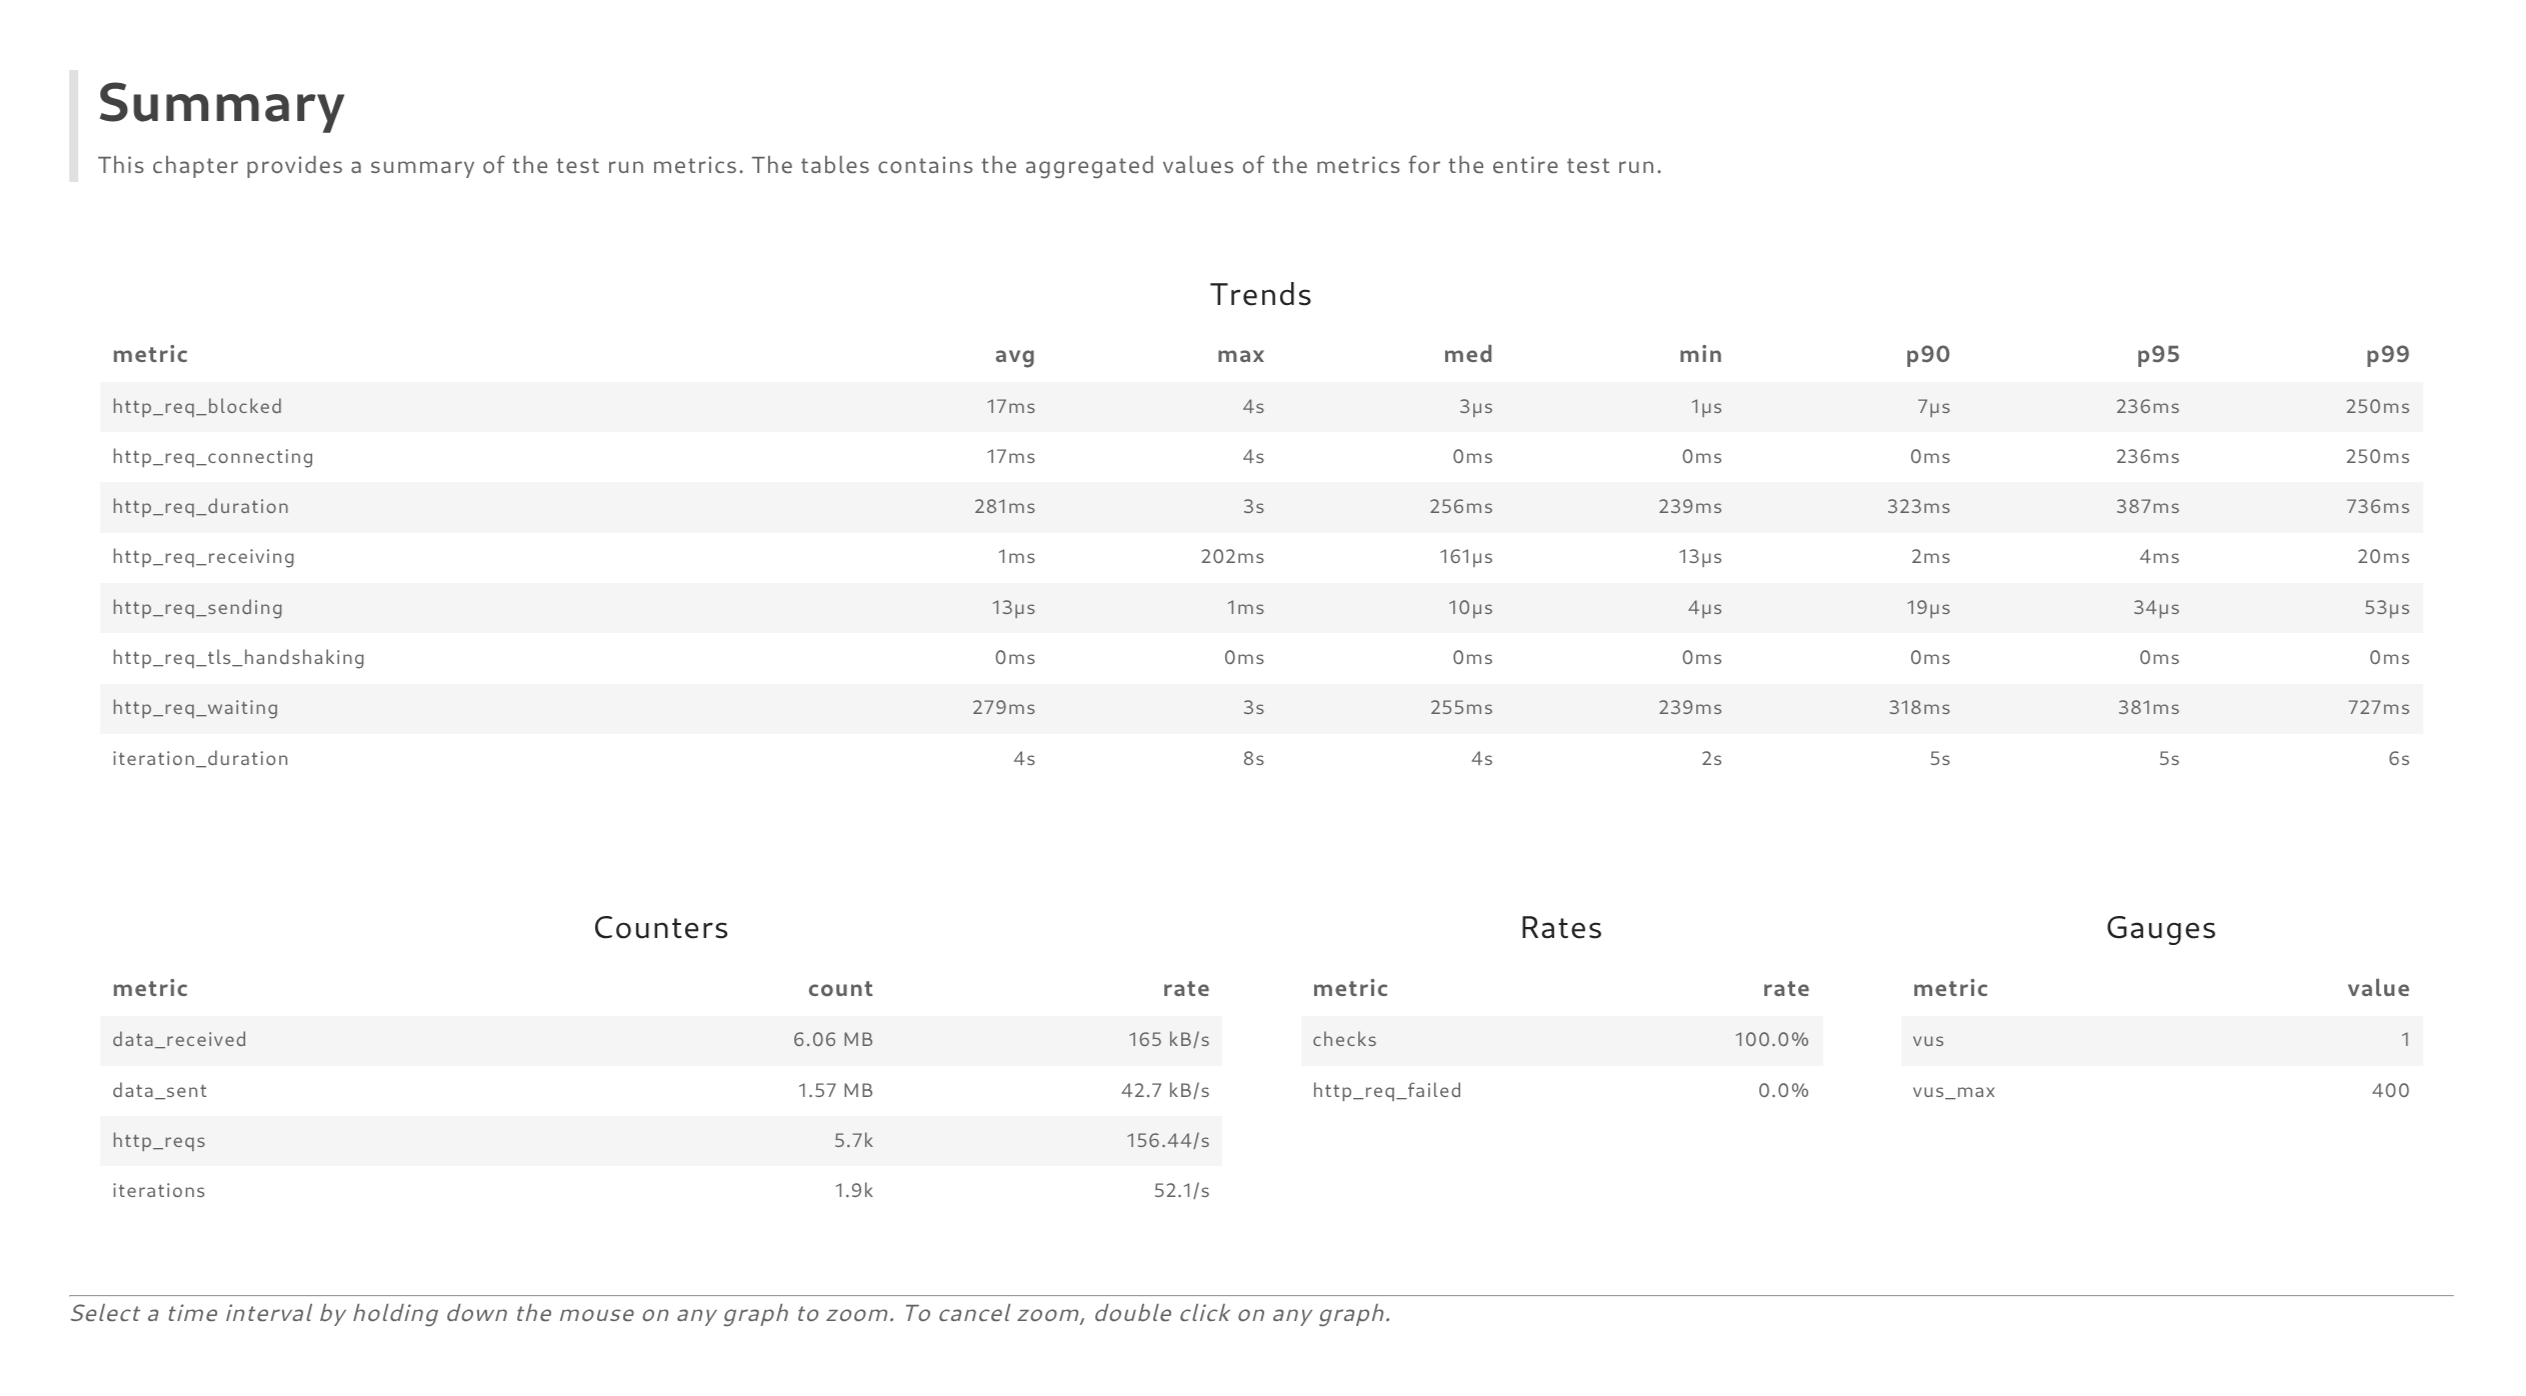
\includegraphics[width=0.98\textwidth]{graphics/chapter-5/5_5_k6/k6_summary_table.png}
    \captionof{figure}{Bảng Summary của K6 sau khi hoàn tất benchmark}
    \label{fig:k6-summary-table}
\end{center}

\noindent Hình \ref{fig:k6-summary-table} tổng hợp các thống kê sau khi chạy xong benchmark. Trong lượt chạy này, \texttt{http\_req\_duration} trung bình vào khoảng \texttt{281ms}, \texttt{p95} đạt \texttt{387ms}, \texttt{p99} lên tới \texttt{736ms} và tỷ lệ lỗi vẫn giữ ở mức \texttt{0.0\%}. Các số liệu này đủ để làm đường cơ sở khi so sánh với những lần chạy có tiêm lỗi ở các phần sau.

\begin{center}
    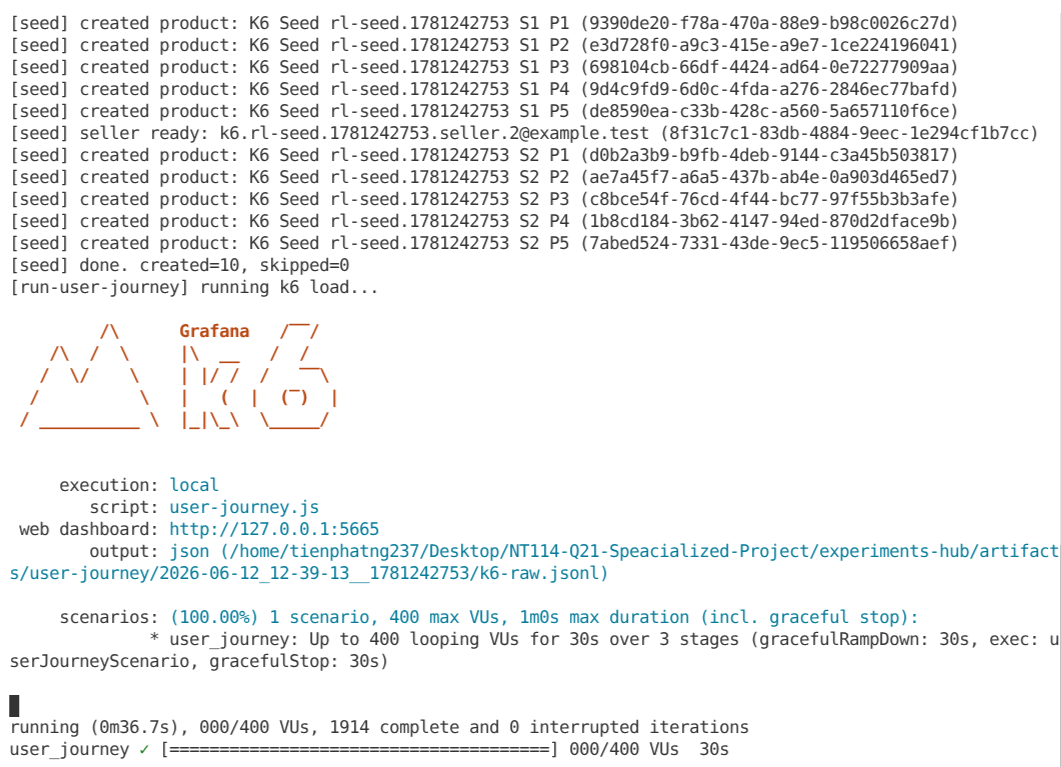
\includegraphics[width=0.98\textwidth]{graphics/chapter-5/5_5_k6/k6_run_log.png}
    \captionof{figure}{Nhật ký thực thi kịch bản K6 và xuất dữ liệu kết quả}
    \label{fig:k6-run-log}
\end{center}

\noindent Hình \ref{fig:k6-run-log} cho thấy quá trình khởi chạy kịch bản, sinh dữ liệu seed và ghi kết quả đầu ra. Sau khi K6 kết thúc, hệ thống xuất dữ liệu thô và dữ liệu tổng hợp theo các mốc thời gian:
\begin{itemize}
    \item \texttt{k6-summary.json}
    \item \texttt{k6-raw.jsonl}
    \item \texttt{combined-report.json}
    \item \texttt{combined-report.csv}
    \item \texttt{combined-report.parquet}
\end{itemize}
\noindent Đặc biệt, bước \texttt{export-combined-report.py} sẽ hợp nhất chỉ số K6 với dữ liệu Prometheus theo bucket 5 giây, tạo thành tập dữ liệu đầu vào trực tiếp cho phân tích hiệu năng và huấn luyện tác nhân RL.

\begin{center}
\captionof{table}{Một số thông số chính trong cấu hình K6 (\texttt{.env.k6.fast})}
\label{tab:k6-fast-profile-config}
\footnotesize
\renewcommand{\arraystretch}{1.0}
\begin{tabular}{|L{4.0cm}|C{3.0cm}|L{7.6cm}|}
\hline
\textbf{Tham số} & \textbf{Giá trị} & \textbf{Ý nghĩa} \\ \hline
\texttt{BASE\_URL} & \texttt{ALB DNS của hệ thống staging} & Địa chỉ endpoint mục tiêu để phát sinh tải thử nghiệm. \\ \hline
\makecell[l]{\texttt{LOGIN\_ENDPOINT}\\\texttt{PRODUCTS\_ENDPOINT}\\\texttt{ORDERS\_ENDPOINT}} & \texttt{/api/v1/...} & Các API chính trong luồng mô phỏng người dùng. \\ \hline
\texttt{VU\_START} & \texttt{100} & Số lượng người dùng ảo ban đầu. \\ \hline
\texttt{VU\_MAX} & \texttt{250} & Mức người dùng ảo cực đại trong profile tải nhanh. \\ \hline
\texttt{VU\_STEP} & \texttt{15} & Bước tăng người dùng ảo theo mỗi chu kỳ tải. \\ \hline
\texttt{VU\_TIME\_UNIT} & \texttt{10s} & Đơn vị thời gian cho mỗi bước tăng tải. \\ \hline
\makecell[l]{\texttt{VU\_RAMP\_DOWN}\\\texttt{\_DURATION}} & \texttt{10s} & Thời gian giảm tải có kiểm soát trước khi kết thúc lượt chạy. \\ \hline
\texttt{CUSTOMER\_COUNT} & \texttt{5} & Số lượng tài khoản khách hàng được sinh sẵn cho mỗi lần test. \\ \hline
\texttt{THINK\_TIME\_MIN/MAX} & \texttt{0.5 / 2.0} & Khoảng thời gian chờ mô phỏng hành vi người dùng giữa các thao tác. \\ \hline
\texttt{REQUEST\_TIMEOUT} & \texttt{30s} & Ngưỡng timeout cho mỗi HTTP request trong kịch bản K6. \\ \hline
\texttt{PROMETHEUS\_URL} & \texttt{10.0.21.10} & IP của Prometheus Server dùng để thu thập metrics cho đánh giá/huấn luyện RL. \\ \hline
\end{tabular}
\end{center}

\subsection{Mô phỏng sự cố trong quá trình sử dụng}

Để đánh giá khả năng tự phục hồi trong điều kiện vận hành thực, Chaos Mesh được sử dụng để tiêm lỗi trong lúc hệ thống đang phục vụ tải từ K6. Quá trình này được điều phối bởi script \texttt{chaos-mesh/scripts/run-chaos.sh}, cho phép chuẩn hóa cùng một quy trình giữa các lần chạy và giữa các loại sự cố khác nhau.

Mỗi lượt thí nghiệm được tổ chức theo 4 pha thời gian:
\begin{itemize}
    \item \textbf{Baseline}: hệ thống chạy ổn định dưới tải.
    \item \textbf{Warm-up}: tăng độ ổn định của tín hiệu trước khi kích hoạt lỗi.
    \item \textbf{Chaos-active}: lỗi được tiêm trực tiếp bằng manifest Chaos Mesh.
    \item \textbf{Recovery}: ngừng tiêm lỗi và quan sát hệ thống phục hồi.
\end{itemize}
\noindent Theo cấu hình hiện tại trong \texttt{.env.chaos}, thời lượng tương ứng là \texttt{20s / 20s / 30s / 20s}. Script đồng thời ghi \texttt{chaos-timeline.json} để đồng bộ mốc sự kiện chaos với dữ liệu metrics ở bước hậu xử lý.

Trong phạm vi đồ án, kịch bản chính phục vụ đánh giá RL được cấu hình như Bảng \ref{tab:chaos-scenarios-main}.

\begin{center}
\captionof{table}{Kịch bản mô phỏng sự cố chính bằng Chaos Mesh}
\label{tab:chaos-scenarios-main}
\footnotesize
\renewcommand{\arraystretch}{1.0}
\begin{tabular}{|L{4.3cm}|L{2.7cm}|L{3.2cm}|L{4.4cm}|}
\hline
\textbf{Kịch bản} & \textbf{Loại lỗi} & \textbf{Thành phần mục tiêu} & \textbf{Thiết lập chính} \\ \hline
\texttt{pod-kill-product} & PodChaos & \texttt{product-service} & \texttt{action=pod-kill}, \texttt{mode=one}, \texttt{duration=30s}. \\ \hline
\end{tabular}
\end{center}

Ngoài chạy đơn lẻ, hệ thống hỗ trợ chạy lặp nhiều lượt bằng \texttt{run-chaos-batch.sh} để thu đủ số episode cho huấn luyện và so sánh. Kết quả mỗi lượt được lưu theo thư mục artifact riêng, giúp truy vết đầy đủ giữa cấu hình sự cố, dữ liệu tải và dữ liệu metrics.

\subsection{Kết quả kiểm thử hệ thống}

Hình \ref{fig:benchmark-no-rl-timeseries} minh họa một lượt benchmark với các pha \textit{baseline}, \textit{warm-up}, \textit{chaos-active} và \textit{recovery} khi hệ thống chưa áp dụng tác nhân RL để ra quyết định phục hồi.

\begin{center}
    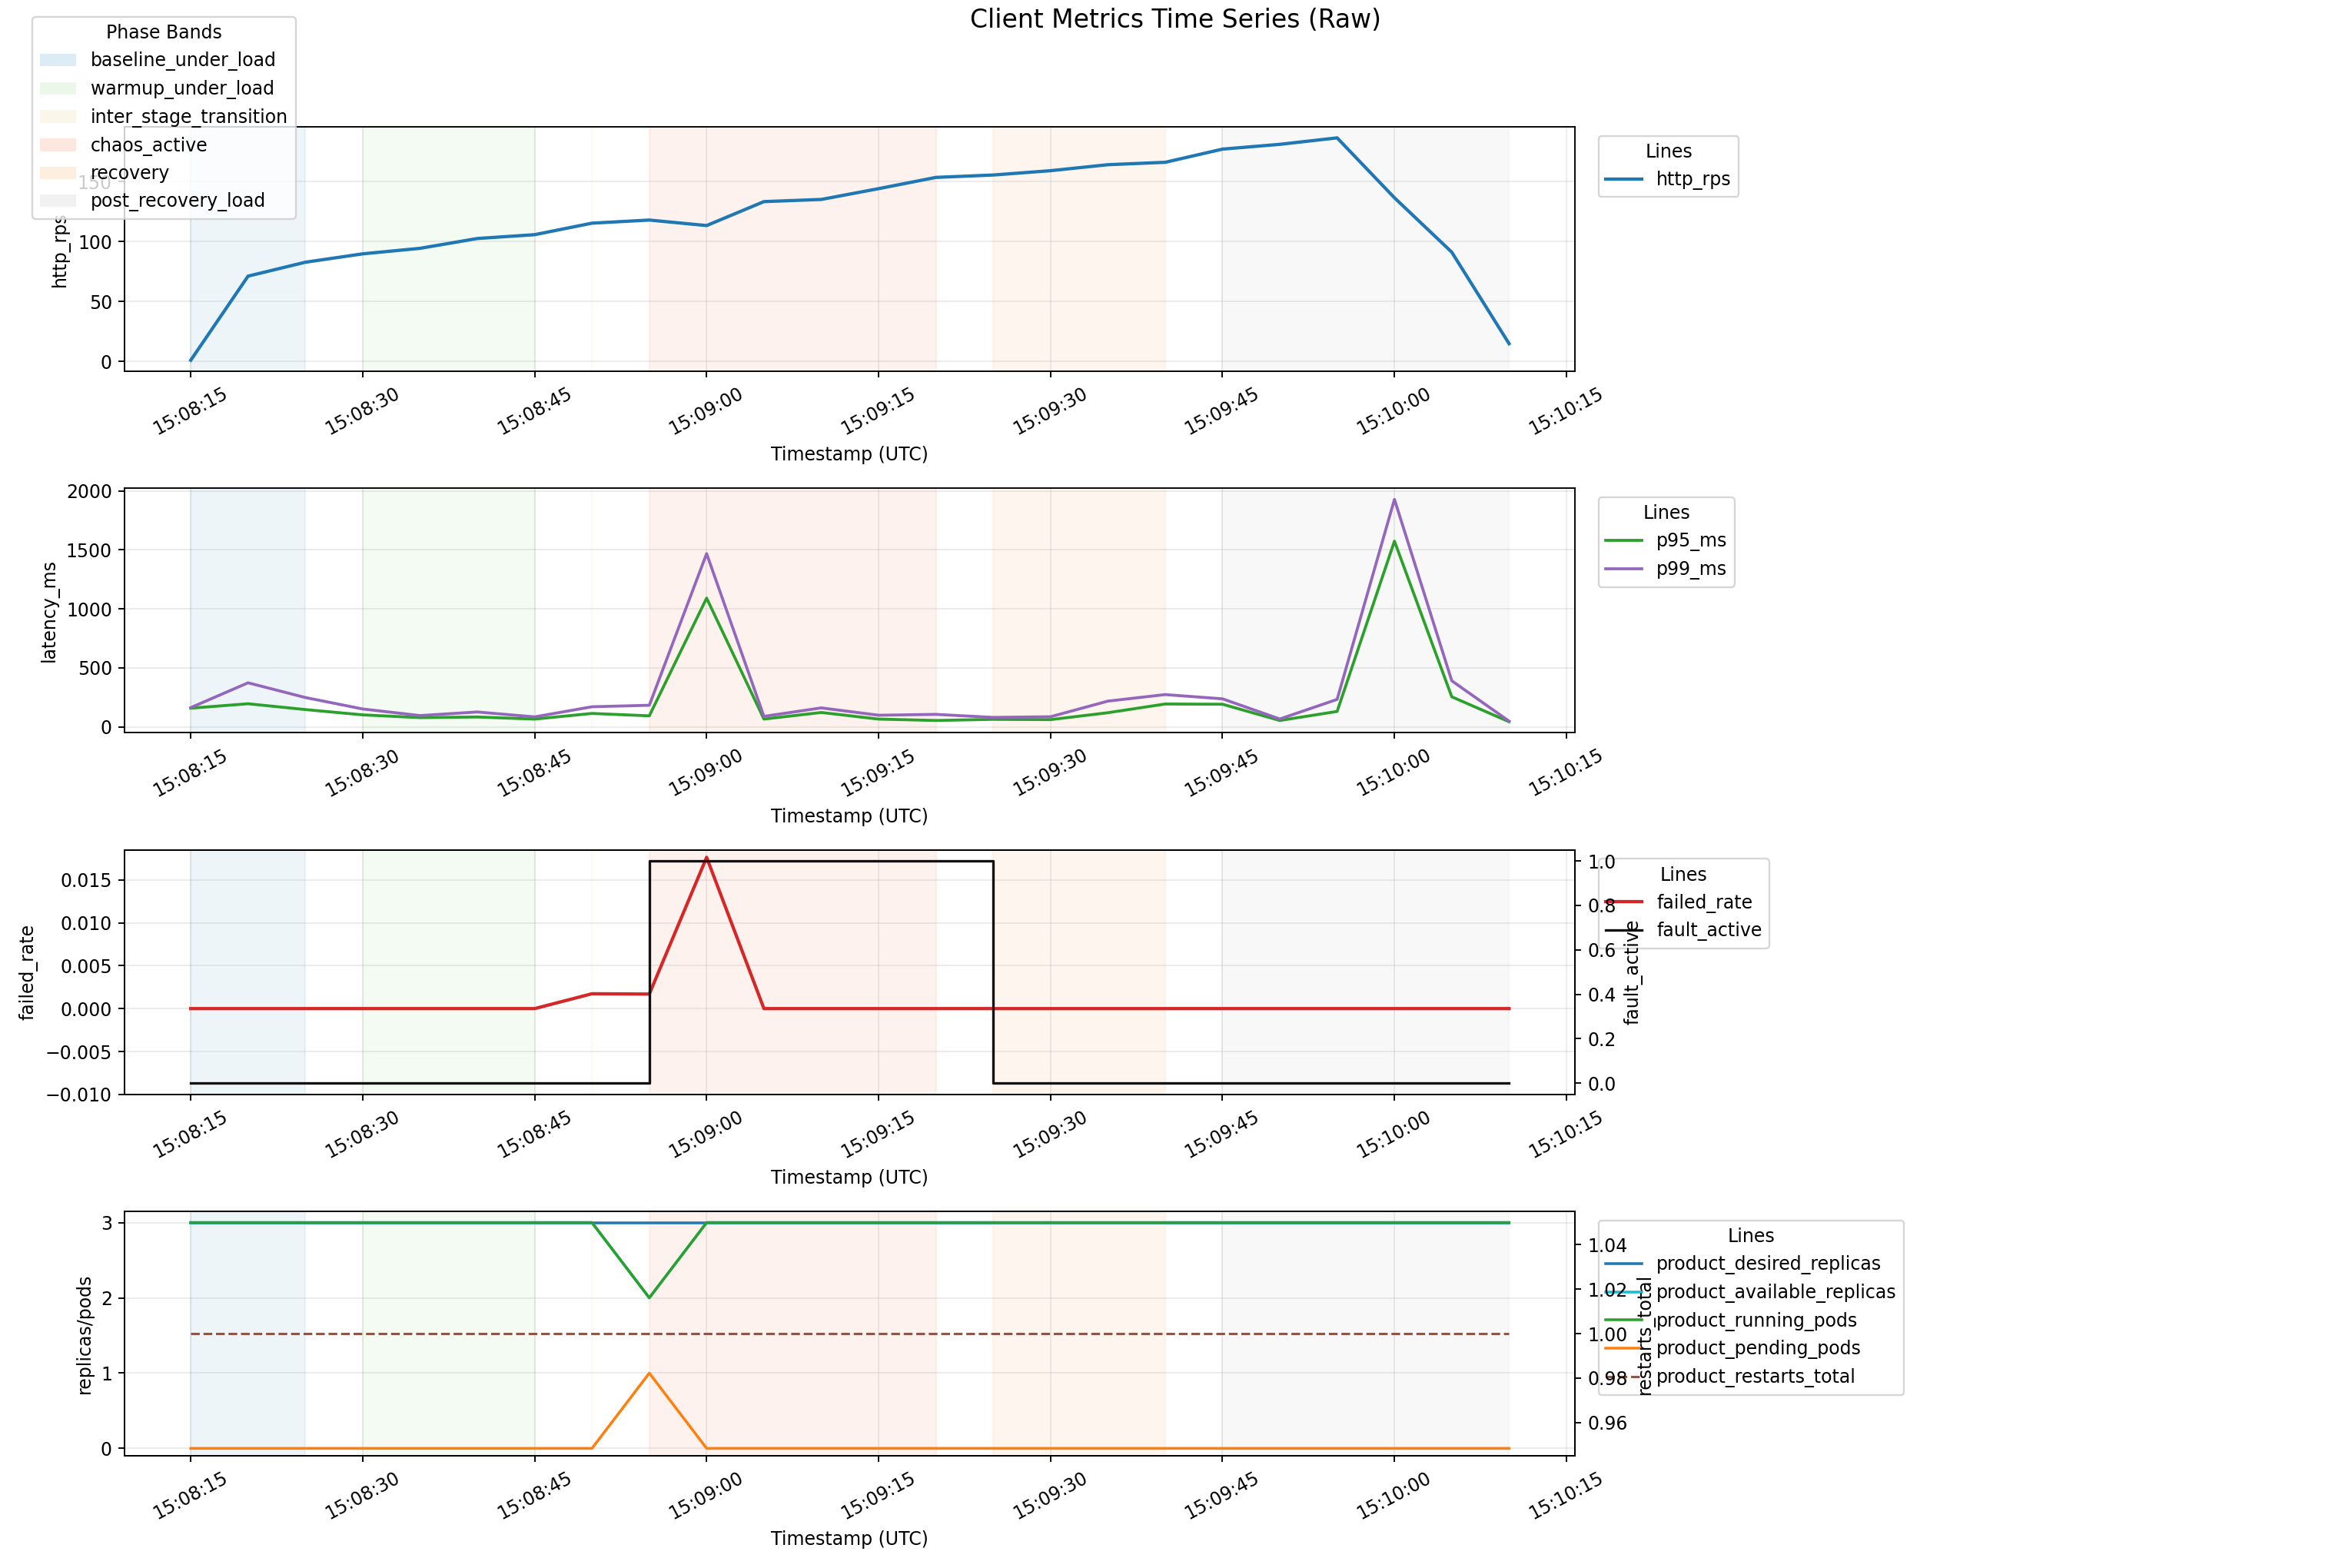
\includegraphics[height=0.5\textheight,keepaspectratio]{graphics/chapter-5/benchmark-norl.png}
    \captionof{figure}{Chuỗi chỉ số phía client và trạng thái workload trong benchmark chưa áp dụng RL}
    \label{fig:benchmark-no-rl-timeseries}
\end{center}

\noindent Từ Hình \ref{fig:benchmark-no-rl-timeseries} có thể quan sát:
\begin{itemize}
    \item Trong pha \textit{chaos-active}, độ trễ p95/p99 xuất hiện các đỉnh tăng mạnh.
    \item \texttt{failed\_rate} tăng ngắn hạn đồng thời với tín hiệu \texttt{fault\_active}.
    \item Số lượng pod \textit{running} có dao động tại thời điểm sự cố trước khi quay về trạng thái ổn định.
\end{itemize}
\noindent Đây là đường cơ sở quan trọng để so sánh mức cải thiện khi áp dụng chính sách tự phục hồi dựa trên RL ở các chương sau.

\begin{center}
    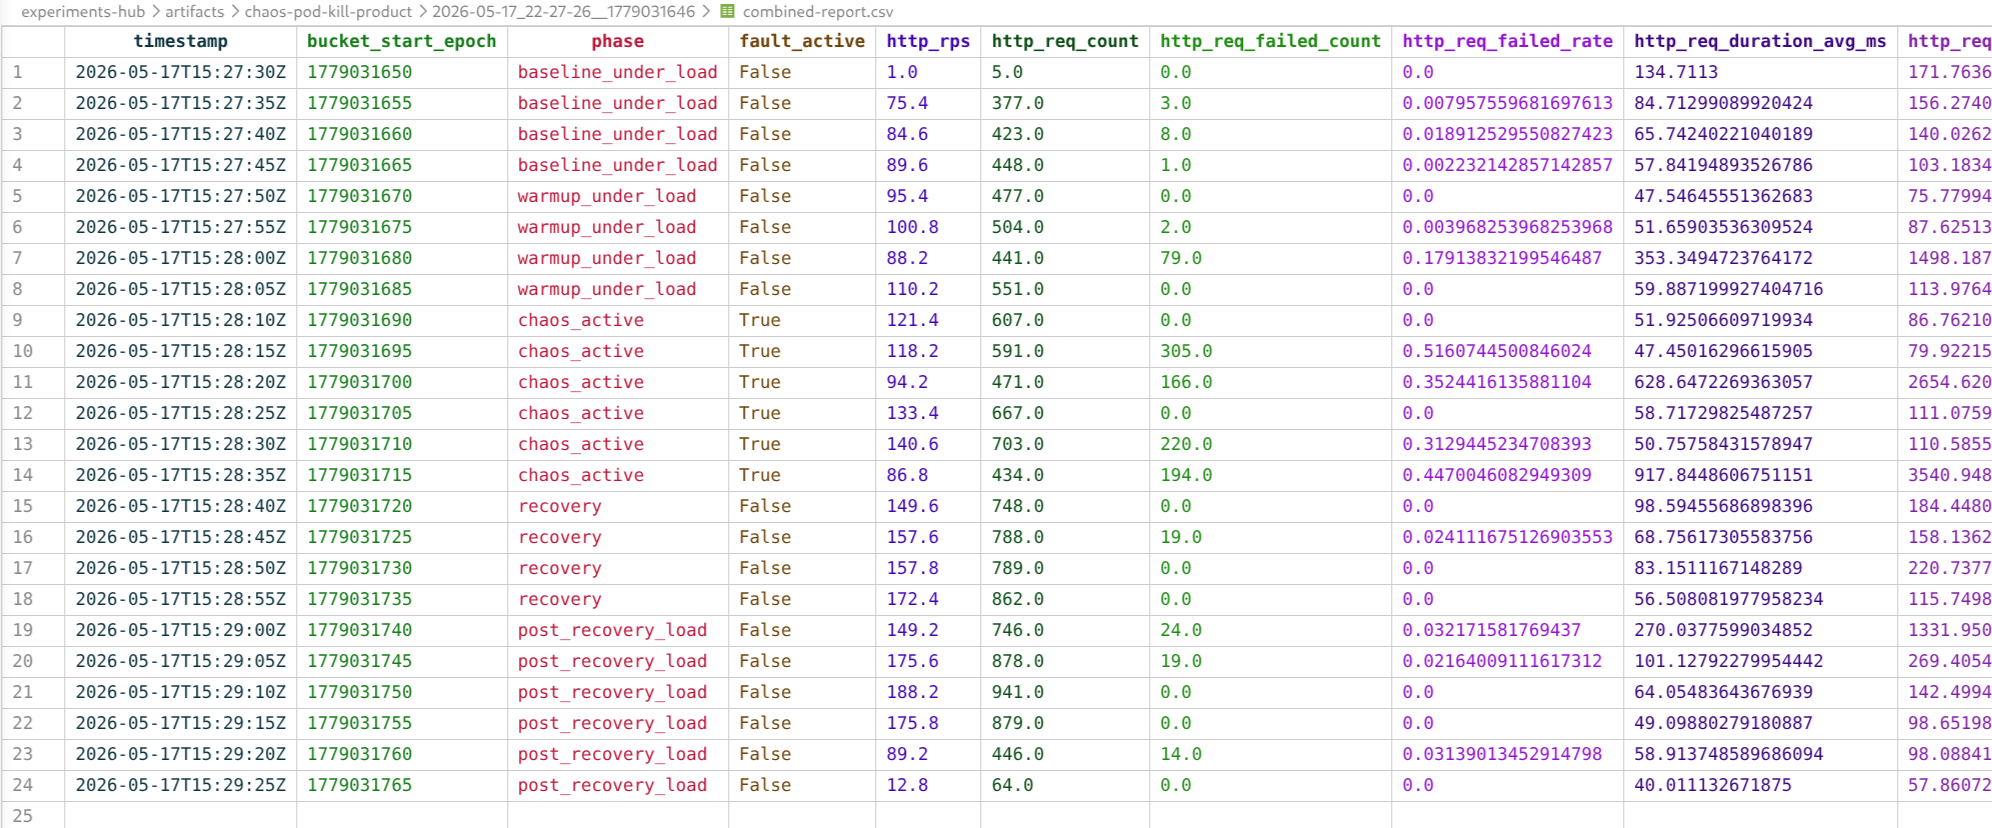
\includegraphics[width=1.0\textwidth]{graphics/chapter-5/metrics.png}
    \captionof{figure}{Trích xuất dữ liệu \texttt{combined-report.csv} sau một lượt chạy benchmark}
    \label{fig:combined-report-csv-snapshot}
\end{center}

\noindent Hình \ref{fig:combined-report-csv-snapshot} cho thấy cấu trúc dữ liệu đầu ra đã được đồng bộ theo bucket 5 giây. Các nhóm trường chính gồm:
\begin{itemize}
    \item Trường thời gian: \texttt{timestamp}, \texttt{bucket\_start\_epoch}.
    \item Trường pha thí nghiệm: \texttt{phase}, \texttt{fault\_active}.
    \item Nhóm chỉ số tải và lỗi:
    \begin{itemize}
        \item \texttt{http\_rps}, \texttt{http\_req\_count}, \texttt{http\_req\_failed\_rate}.
    \end{itemize}
    \item Nhóm chỉ số độ trễ: \texttt{http\_req\_duration\_avg\_ms}, p95, p99.
\end{itemize}
\noindent Cấu trúc này giúp theo dõi biến động hệ thống theo từng pha \textit{baseline}, \textit{chaos-active}, \textit{recovery} và là đầu vào trực tiếp cho bước huấn luyện RL.

\section{Thiết lập huấn luyện RL}

Dữ liệu huấn luyện được lấy từ các tệp \texttt{combined-report.csv} sinh ra sau mỗi lượt chạy benchmark có tải và có tiêm lỗi. Mỗi mẫu dữ liệu đã được đồng bộ theo bucket 5 giây, giữ đầy đủ ngữ cảnh pha thí nghiệm (\textit{baseline}, \textit{warm-up}, \textit{chaos-active}, \textit{recovery}) cùng các chỉ số tải, lỗi và độ trễ.

Trong phạm vi đồ án, quá trình huấn luyện tập trung vào kịch bản \textbf{Pod Failure}, sử dụng dữ liệu từ thí nghiệm \texttt{chaos-pod-kill-product}.

\subsection{Huấn luyện tác nhân DQN}

Đối với DQN, dữ liệu artifact được nạp thành nhiều quỹ đạo trạng thái. Sau đó, môi trường \texttt{ArtifactReplayEnv} được khởi tạo để mô phỏng lại diễn biến của hệ thống theo từng episode, đồng thời cho phép hành động của tác nhân tác động lên trạng thái kế tiếp. Tác nhân DQN sử dụng chính sách \textit{epsilon-greedy}, kết hợp \textit{replay buffer} và \textit{target network} để ổn định quá trình cập nhật giá trị Q.

Các siêu tham số huấn luyện được cấu hình tập trung và được hiệu chỉnh lại theo từng lượt chạy thực nghiệm. Trong cấu hình DQN dùng cho kịch bản \textit{Pod Failure}, các tham số chính được trình bày trong Bảng \ref{tab:dqn-hyperparameters}.

\begin{center}
\captionof{table}{Một số siêu tham số chính trong cấu hình huấn luyện DQN}
\label{tab:dqn-hyperparameters}
\footnotesize
\renewcommand{\arraystretch}{1.0}
\begin{tabular}{|L{4.9cm}|C{2.3cm}|L{7.6cm}|}
\hline
\textbf{Tham số} & \textbf{Giá trị} & \textbf{Vai trò} \\ \hline
\texttt{timesteps} & \texttt{400000} & Tổng số bước huấn luyện của tác nhân DQN trên môi trường replay. \\ \hline
\texttt{eval\_episodes} & \texttt{40} & Số episode dùng để đánh giá định kỳ sau huấn luyện. \\ \hline
\texttt{max\_steps} & \texttt{80} & Giới hạn số bước tối đa trong mỗi episode. \\ \hline
\texttt{learning\_rate} & \texttt{5e-5} & Tốc độ cập nhật trọng số của mạng Q chính. \\ \hline
\texttt{buffer\_size} & \texttt{200000} & Kích thước bộ nhớ kinh nghiệm dùng để lưu các mẫu chuyển trạng thái. \\ \hline
\texttt{learning\_starts} & \texttt{10000} & Số bước tích lũy ban đầu trước khi bắt đầu cập nhật mạng Q. \\ \hline
\texttt{batch\_size} & \texttt{256} & Số mẫu được lấy trong mỗi lần cập nhật mini-batch. \\ \hline
\texttt{gamma} & \texttt{0.995} & Hệ số chiết khấu, ưu tiên phần thưởng dài hạn trong quá trình học. \\ \hline
\makecell[l]{\texttt{train\_freq}\\\texttt{gradient\_steps}} & \texttt{4 / 2} & Chu kỳ lấy mẫu cập nhật và số bước tối ưu hóa được thực hiện sau mỗi lần học. \\ \hline
\makecell[l]{\texttt{target\_update\_}\\\texttt{interval}} & \texttt{2000} & Chu kỳ đồng bộ từ mạng Q chính sang mạng mục tiêu để giảm dao động. \\ \hline
\makecell[l]{\texttt{exploration\_initial\_eps}\\to \texttt{exploration\_final\_eps}} & \texttt{1.0 -> 0.05} & Lịch giảm epsilon trong chiến lược \textit{epsilon-greedy}, chuyển dần từ khám phá sang khai thác. \\ \hline
\makecell[l]{\texttt{exploration\_}\\\texttt{fraction}} & \texttt{0.25} & Tỷ lệ tiến trình huấn luyện dành cho giai đoạn giảm epsilon. \\ \hline
\texttt{rolling\_window} & \texttt{40} & Cửa sổ làm mượt dùng khi theo dõi đường hội tụ trong quá trình huấn luyện. \\ \hline
\texttt{dynamics\_mode} & \makecell[c]{\texttt{hybrid\_}\\\texttt{controlled}} & Chế độ mô phỏng động học môi trường khi replay từ dữ liệu artifact. \\ \hline
\texttt{noise\_scale} & \texttt{0.7} & Mức nhiễu bổ sung nhằm tránh tác nhân học quá khớp với một quỹ đạo cố định. \\ \hline
\texttt{seed} & \texttt{42} & Hạt giống ngẫu nhiên để tái lập thí nghiệm. \\ \hline
\end{tabular}
\end{center}

Trong quá trình huấn luyện, mô hình được theo dõi thông qua các chỉ số như phần thưởng theo episode, epsilon, loss và hiệu quả đánh giá sau huấn luyện. Kết quả mỗi lượt chạy được lưu dưới dạng mô hình DQN, các biểu đồ hội tụ và tệp metadata, làm cơ sở cho bước so sánh ở Chương 6.

\subsection{Huấn luyện tác nhân A2C}

Đối với A2C, dữ liệu artifact cũng được nạp thành nhiều quỹ đạo trạng thái và replay trên môi trường \texttt{ArtifactReplayEnv} để tái hiện diễn biến của hệ thống theo từng episode. Khác với DQN, A2C tối ưu đồng thời mạng chính sách (actor) và mạng giá trị (critic), nhờ đó tác nhân học trực tiếp phân phối hành động trên tập hành động rời rạc gồm \texttt{idle}, \texttt{restart\_pod}, \texttt{scale\_up} và \texttt{scale\_down}. Cách tiếp cận này phù hợp với bài toán self-healing khi cần giữ cân bằng giữa khả năng khám phá và độ ổn định của cập nhật trên dữ liệu benchmark có nhiễu.

Các siêu tham số huấn luyện được cấu hình tập trung và được hiệu chỉnh lại theo từng lượt chạy thực nghiệm. Trong cấu hình A2C dùng cho kịch bản \textit{Pod Failure}, các tham số chính được trình bày trong Bảng \ref{tab:a2c-hyperparameters}.

\begin{center}
\captionof{table}{Một số siêu tham số chính trong cấu hình huấn luyện A2C}
\label{tab:a2c-hyperparameters}
\footnotesize
\renewcommand{\arraystretch}{1.0}
\begin{tabular}{|L{4.0cm}|C{2.3cm}|L{8.7cm}|}
\hline
\textbf{Tham số} & \textbf{Giá trị} & \textbf{Vai trò} \\ \hline
\texttt{timesteps} & \texttt{300000} & Tổng số bước huấn luyện của tác nhân A2C trên môi trường replay. \\ \hline
\texttt{eval\_episodes} & \texttt{40} & Số episode dùng để đánh giá định kỳ sau huấn luyện. \\ \hline
\texttt{max\_steps} & \texttt{80} & Giới hạn số bước tối đa trong mỗi episode. \\ \hline
\texttt{min\_traj\_len} & \texttt{20} & Độ dài quỹ đạo tối thiểu để một đoạn dữ liệu được dùng cho huấn luyện. \\ \hline
\texttt{learning\_rate} & \texttt{1e-4} & Tốc độ cập nhật tham số cho actor và critic. \\ \hline
\texttt{n\_steps} & \texttt{64} & Số bước rollout được thu thập trước mỗi lần cập nhật A2C. \\ \hline
\texttt{gamma} & \texttt{0.995} & Hệ số chiết khấu, nhấn mạnh lợi ích dài hạn của chuỗi phục hồi. \\ \hline
\texttt{gae\_lambda} & \texttt{0.97} & Tham số làm trơn ước lượng advantage để giảm phương sai. \\ \hline
\texttt{ent\_coef} & \texttt{0.001} & Hệ số entropy giúp duy trì mức khám phá phù hợp trong giai đoạn đầu. \\ \hline
\texttt{vf\_coef} & \texttt{0.5} & Trọng số của hàm mất mát giá trị trong tối ưu tổng thể. \\ \hline
\texttt{rolling\_window} & \texttt{40} & Cửa sổ làm mượt dùng khi theo dõi đường hội tụ trong quá trình huấn luyện. \\ \hline
\texttt{dynamics\_mode} & \makecell[c]{\texttt{hybrid\_}\\\texttt{controlled}} & Chế độ mô phỏng động học môi trường khi replay từ dữ liệu artifact. \\ \hline
\texttt{noise\_scale} & \texttt{0.65} & Mức nhiễu bổ sung giúp tác nhân tránh học quá khớp theo một quỹ đạo cố định. \\ \hline
\texttt{seed} & \texttt{42} & Hạt giống ngẫu nhiên để tái lập thí nghiệm. \\ \hline
\end{tabular}
\end{center}

Trong quá trình huấn luyện, mô hình A2C được theo dõi thông qua phần thưởng theo episode, độ dài episode, entropy và hiệu quả đánh giá sau huấn luyện. Kết quả mỗi lượt chạy được lưu dưới dạng mô hình A2C, các biểu đồ hội tụ và tệp metadata, làm cơ sở cho bước so sánh với DQN, PPO và baseline ở Chương 6.

\subsection{Huấn luyện tác nhân PPO}

Với PPO, cùng một tập trajectory và cùng môi trường \texttt{ArtifactReplayEnv} được sử dụng để bảo đảm so sánh công bằng với DQN. Mô hình học trực tiếp chính sách trên không gian trạng thái đã được ánh xạ từ dữ liệu benchmark, nhờ đó phù hợp với bài toán phục hồi theo chuỗi quyết định liên tục qua từng bước thời gian.

Các siêu tham số huấn luyện được cấu hình tập trung và được hiệu chỉnh lại theo từng lượt chạy thực nghiệm. Trong cấu hình PPO dùng cho kịch bản \textit{Pod Failure}, các tham số chính được trình bày trong Bảng \ref{tab:ppo-hyperparameters}.

\begin{center}
\captionof{table}{Một số siêu tham số chính trong cấu hình huấn luyện PPO}
\label{tab:ppo-hyperparameters}
\footnotesize
\renewcommand{\arraystretch}{1.0}
\begin{tabular}{|L{4.3cm}|C{2.3cm}|L{7.9cm}|}
\hline
\textbf{Tham số} & \textbf{Giá trị} & \textbf{Vai trò} \\ \hline
\texttt{timesteps} & \texttt{400000} & Tổng số bước huấn luyện của tác nhân PPO trên môi trường replay. \\ \hline
\texttt{eval\_episodes} & \texttt{40} & Số episode dùng để đánh giá định kỳ sau huấn luyện. \\ \hline
\texttt{max\_steps} & \texttt{80} & Giới hạn số bước tối đa trong mỗi episode huấn luyện. \\ \hline
\texttt{min\_traj\_len} & \texttt{20} & Độ dài quỹ đạo tối thiểu để một đoạn dữ liệu được dùng cho huấn luyện. \\ \hline
\texttt{learning\_rate} & \texttt{1e-4} & Tốc độ cập nhật tham số của mạng chính sách và mạng giá trị. \\ \hline
\texttt{n\_steps} & \texttt{2048} & Số bước rollout được thu thập trước mỗi lần cập nhật PPO. \\ \hline
\texttt{batch\_size} & \texttt{128} & Kích thước mini-batch dùng khi tối ưu trên dữ liệu rollout. \\ \hline
\texttt{gamma} & \texttt{0.995} & Hệ số chiết khấu cho phần thưởng dài hạn trong quá trình học. \\ \hline
\texttt{gae\_lambda} & \texttt{0.97} & Hệ số GAE giúp ước lượng advantage ổn định hơn. \\ \hline
\texttt{rolling\_window} & \texttt{40} & Cửa sổ làm mượt dùng khi theo dõi đường hội tụ trong quá trình huấn luyện. \\ \hline
\texttt{dynamics\_mode} & \makecell[c]{\texttt{hybrid\_}\\\texttt{controlled}} & Chế độ mô phỏng động học môi trường khi replay từ dữ liệu artifact. \\ \hline
\texttt{noise\_scale} & \texttt{0.65} & Mức nhiễu bổ sung nhằm tránh tác nhân học quá khớp theo một quỹ đạo cố định. \\ \hline
\texttt{seed} & \texttt{42} & Hạt giống ngẫu nhiên để tái lập thí nghiệm. \\ \hline
\end{tabular}
\end{center}

Sau khi hoàn tất huấn luyện, tác nhân PPO được đánh giá trên nhiều episode và đối chiếu với tác nhân baseline ngẫu nhiên. Kết quả mỗi lượt chạy được lưu dưới dạng mô hình PPO, các biểu đồ hội tụ và tệp metadata, từ đó hỗ trợ phân tích khả năng phục hồi và mức độ ổn định của chính sách học được.

\section{Triển khai mô hình RL trên Kubernetes}

Sau giai đoạn huấn luyện, mô hình RL được đóng gói và đưa trở lại môi trường vận hành dưới dạng các dịch vụ chạy thường trực trên cụm Kubernetes \texttt{k0s}. Cụm này được triển khai trong các private subnet của AWS VPC, nhờ đó toàn bộ thành phần suy luận và thực thi self-healing được đặt gần workload mục tiêu nhưng vẫn giữ nguyên nguyên tắc cô lập mạng và kiểm soát truy cập. Ứng dụng đích trong phạm vi đồ án là hệ thống \texttt{mini-ecommerce}, bao gồm các service \texttt{api-gateway}, \texttt{user-service}, \texttt{inventory-service}, \texttt{order-service}, \texttt{product-service} và \texttt{payment-service}.

Về mặt logic, lớp suy luận RL được bố trí trong namespace riêng \texttt{rl-agent}, tách biệt khỏi namespace ứng dụng nghiệp vụ nhưng vẫn có khả năng quan sát và can thiệp có kiểm soát lên workload mục tiêu thông qua Kubernetes API. Mô hình triển khai này giúp quá trình giám sát, suy luận và thực thi hành động phục hồi diễn ra liên tục trong cùng môi trường thí nghiệm, đồng thời thuận tiện cho việc mở rộng, thay thế phiên bản mô hình hoặc giới hạn phạm vi tác động của tác nhân RL.

\subsection{Kiến trúc triển khai RL Agent}

Kiến trúc triển khai của lớp self-healing dựa trên RL được tổ chức thành ba tầng chức năng: thu thập trạng thái, suy luận chính sách và thực thi hành động. Ở tầng đầu vào, Pod \texttt{metrics-collector} kết nối tới Prometheus và Kubernetes API để lấy các chỉ số vận hành cốt lõi của hệ thống. Các chỉ số này sau đó được chuẩn hóa thành vector trạng thái dùng cho mô hình RL. Ở tầng suy luận, Deployment \texttt{rl-agent} duy trì đồng thời ba bản sao nhằm tăng tính sẵn sàng và hạn chế điểm lỗi đơn lẻ cho thành phần ra quyết định. Ở tầng thực thi, Pod \texttt{action-executor} nhận hành động từ RL Agent và gửi lệnh can thiệp tới Kubernetes API Server.

\noindent Luồng xử lý tổng quát của hệ thống có thể được biểu diễn như sau:

\begin{center}
    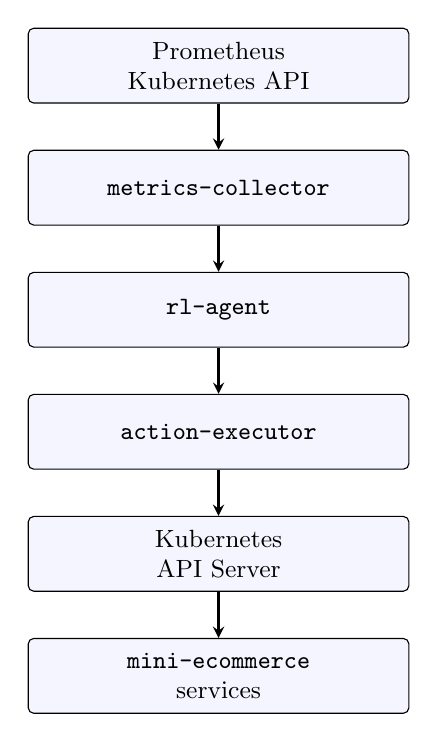
\begin{tikzpicture}[
        >=stealth,
        every node/.style={font=\small},
        flowbox/.style={
            draw,
            rounded corners=2pt,
            align=center,
            minimum height=0.95cm,
            text width=4.6cm,
            fill=blue!4
        }
    ]
        \node[flowbox] (source) at (0,0) {Prometheus\\Kubernetes API};
        \node[flowbox] (collector) at (0,-1.55) {\texttt{metrics-collector}};
        \node[flowbox] (agent) at (0,-3.10) {\texttt{rl-agent}};
        \node[flowbox] (executor) at (0,-4.65) {\texttt{action-executor}};
        \node[flowbox] (apiserver) at (0,-6.20) {Kubernetes\\API Server};
        \node[flowbox] (services) at (0,-7.75) {\texttt{mini-ecommerce}\\services};

        \draw[->, thick] (source) -- (collector);
        \draw[->, thick] (collector) -- (agent);
        \draw[->, thick] (agent) -- (executor);
        \draw[->, thick] (executor) -- (apiserver);
        \draw[->, thick] (apiserver) -- (services);
    \end{tikzpicture}
\end{center}

\noindent Cách bố trí này phù hợp với đặc thù của bài toán self-healing vì nó tách riêng quá trình quan sát trạng thái và thực thi hành động khỏi chính workload mục tiêu. Nhờ đó, ngay cả khi một dịch vụ trong \texttt{mini-ecommerce} gặp lỗi hoặc mất ổn định, lớp điều phối RL vẫn có khả năng tiếp tục hoạt động và đưa ra quyết định phục hồi.

\subsection{Các thành phần chính}

Trong cấu hình hiện tại, lớp RL Agent được triển khai thành tổng cộng năm Pod chính, bao gồm một Pod \texttt{metrics-collector}, ba Pod \texttt{rl-agent} và một Pod \texttt{action-executor}. Vai trò của từng Pod được tóm tắt trong Bảng \ref{tab:rl-agent-pods}.

\begin{center}
\captionof{table}{Các Pod chính trong lớp triển khai RL trên Kubernetes}
\label{tab:rl-agent-pods}
\footnotesize
\renewcommand{\arraystretch}{1.1}
\begin{tabular}{|L{3.2cm}|C{1.8cm}|L{3.1cm}|L{6.5cm}|}
\hline
\textbf{Thành phần} & \textbf{Số Pod} & \textbf{Vai trò chính} & \textbf{Mô tả} \\ \hline
\texttt{metrics-collector} & 1 & Thu thập trạng thái & Lấy metrics từ Prometheus và Kubernetes API, gồm CPU usage, memory usage, request latency p95, error rate, restart count và replica count; sau đó chuyển đổi thành state đầu vào cho mô hình RL. \\ \hline
\texttt{rl-agent} & 3 & Suy luận chính sách & Mỗi Pod nạp mô hình đã huấn luyện, nhận state từ \texttt{metrics-collector} và suy luận một action thuộc tập \texttt{idle}, \texttt{restart pod}, \texttt{scale up}, \texttt{scale down}. Việc duy trì ba replica giúp tăng tính sẵn sàng và khả năng chịu lỗi của thành phần ra quyết định. \\ \hline
\texttt{action-executor} & 1 & Thực thi hành động & Nhận action từ RL Agent, gọi Kubernetes API để \texttt{rollout restart} Deployment, xóa Pod lỗi hoặc thay đổi số replica của Deployment mục tiêu. \\ \hline
\end{tabular}
\end{center}

\noindent Trong ba thành phần trên, \texttt{metrics-collector} đóng vai trò cầu nối giữa lớp observability và mô hình RL. Thành phần này không chỉ lấy dữ liệu thô mà còn thực hiện bước gom nhóm theo cửa sổ thời gian, chuẩn hóa đơn vị đo và ánh xạ các chỉ số sang đúng thứ tự đặc trưng mà mô hình đã sử dụng khi huấn luyện. Điều này giúp giảm sai khác giữa môi trường huấn luyện và môi trường triển khai thực tế.

\noindent Đối với \texttt{rl-agent}, việc triển khai theo dạng Deployment với \texttt{replicas: 3} thay vì chỉ một Pod duy nhất nhằm tránh trường hợp lớp ra quyết định trở thành điểm lỗi đơn. Trong ngữ cảnh self-healing, đây là yêu cầu quan trọng vì khi hệ thống đích đang chịu lỗi, thành phần điều phối phục hồi cần duy trì được khả năng suy luận và phản hồi ổn định.

\noindent Minh họa cấu hình Deployment của \texttt{rl-agent} được trình bày như sau:
\begin{lstlisting}
apiVersion: apps/v1
kind: Deployment
metadata:
  name: rl-agent
  namespace: rl-agent
spec:
  replicas: 3
  selector:
    matchLabels:
      app: rl-agent
  template:
    metadata:
      labels:
        app: rl-agent
    spec:
      serviceAccountName: rl-agent-sa
      containers:
        - name: rl-agent
          image: rl-agent:latest
          env:
            - name: PROMETHEUS_URL
              value: "http://prometheus.monitoring:9090"
            - name: TARGET_NAMESPACE
              value: "mini-ecommerce"
            - name: ACTION_SPACE
              value: "idle,restart,scale_up,scale_down"
          resources:
            requests:
              cpu: "100m"
              memory: "256Mi"
            limits:
              cpu: "500m"
              memory: "1Gi"



\end{lstlisting}

\subsection{Luồng hoạt động self-healing}

Trong quá trình vận hành, các dịch vụ của hệ thống \texttt{mini-ecommerce} liên tục sinh ra dữ liệu quan sát về tài nguyên, độ trễ và tỷ lệ lỗi. Prometheus thu thập các số liệu này theo chu kỳ và lưu trữ dưới dạng time series. Song song với đó, Kubernetes API cung cấp thông tin bổ sung về số replica, trạng thái Pod, số lần restart và các sự kiện vòng đời quan trọng khác.

\noindent Pod \texttt{metrics-collector} định kỳ truy vấn hai nguồn dữ liệu trên để xây dựng trạng thái hiện thời của hệ thống. Trạng thái này phản ánh cả mức tiêu thụ tài nguyên lẫn chất lượng phục vụ của ứng dụng, từ đó tạo đầu vào phù hợp cho bài toán quyết định trong self-healing. Sau khi nhận được state, mỗi Pod \texttt{rl-agent} thực hiện bước suy luận dựa trên policy của mô hình đã được huấn luyện trước đó. Kết quả suy luận là một action trong không gian hành động rời rạc, gồm giữ nguyên trạng thái (\texttt{idle}), khởi động lại Pod lỗi (\texttt{restart pod}), tăng số lượng bản sao (\texttt{scale up}) hoặc giảm số lượng bản sao (\texttt{scale down}).

\noindent Action sau đó được chuyển sang \texttt{action-executor}. Thành phần này đóng vai trò trung gian để tách riêng phần suy luận ra khỏi phần can thiệp hạ tầng. Cách thiết kế này giúp giới hạn bề mặt tấn công của RL Agent, đồng thời cho phép bổ sung thêm các bước kiểm tra an toàn trước khi gửi lệnh xuống Kubernetes API Server. Sau khi hành động được thực thi, trạng thái mới của hệ thống tiếp tục được Prometheus và Kubernetes API ghi nhận, tạo thành vòng lặp quan sát -- quyết định -- can thiệp -- đánh giá liên tục.

\subsection{Cơ chế thực thi action trên Kubernetes}

Từ góc độ triển khai, \texttt{action-executor} là thành phần duy nhất trực tiếp gọi Kubernetes API để thay đổi trạng thái workload. Khi action đầu ra là \texttt{restart pod}, executor có thể chọn một trong hai cách tiếp cận: yêu cầu \texttt{rollout restart} đối với Deployment mục tiêu hoặc xóa trực tiếp Pod đang lỗi để ReplicaSet tạo lại bản sao mới. Khi action là \texttt{scale up} hoặc \texttt{scale down}, executor sẽ cập nhật trường \texttt{spec.replicas} của Deployment tương ứng. Trong trường hợp action là \texttt{idle}, hệ thống chỉ ghi log quyết định và tiếp tục vòng quan sát kế tiếp.

\noindent Để tránh việc tác nhân RL có quyền thao tác quá rộng, cơ chế thực thi được ràng buộc bằng \texttt{ServiceAccount}, \texttt{Role} và \texttt{RoleBinding}. Các quyền này chỉ nên giới hạn trong namespace ứng dụng \texttt{mini-ecommerce} và tập tài nguyên thật sự cần thiết, chủ yếu là \texttt{pods}, \texttt{deployments} và \texttt{deployments/scale}. Cách tiếp cận tối thiểu quyền hạn này giúp giảm rủi ro can thiệp ngoài ý muốn vào các namespace hạ tầng hoặc thành phần quan sát.

\newpage
\noindent Ví dụ rút gọn cho cấu hình quyền thực thi như sau:
\begin{lstlisting}
apiVersion: rbac.authorization.k8s.io/v1
kind: Role
metadata:
  name: rl-agent-role
  namespace: mini-ecommerce
rules:
  - apiGroups: [""]
    resources: ["pods"]
    verbs: ["get", "list", "watch", "delete"]
  - apiGroups: ["apps"]
    resources: ["deployments", "deployments/scale"]
    verbs: ["get", "list", "watch", "patch", "update"]
\end{lstlisting}

\noindent Bên cạnh RBAC, lớp executor cũng có thể áp dụng thêm các guardrail như giới hạn số replica tối thiểu/tối đa, thời gian chờ giữa hai lần can thiệp liên tiếp và cơ chế bỏ qua action nếu trạng thái hệ thống chưa ổn định. Những ràng buộc này không thay thế mô hình RL, nhưng giúp quá trình triển khai thực tế an toàn và nhất quán hơn.

\noindent Tóm lại, mục này tập trung vào cách tổ chức và triển khai lớp RL Agent lên cụm \texttt{k0s} dưới dạng các Pod chuyên biệt cho thu thập trạng thái, suy luận chính sách và thực thi hành động. Cách bố trí này giúp mô hình đã huấn luyện có thể vận hành trực tiếp trong môi trường Kubernetes, đồng thời giữ được tính tách biệt với workload nghiệp vụ và khả năng kiểm soát quyền can thiệp thông qua các cơ chế chuẩn của nền tảng.
